\documentclass[a4paper,twoside,12pt]{report}
% Marcell Nagy (2022)

% Include Packages
\usepackage[a4paper,inner=3.5cm,outer=2.5cm,top=2.5cm,bottom=2.5cm]{geometry}  % Set page margins
\usepackage{fullpage}
\usepackage{float}                  % Allows 'Here and Only Here' [H] for Floats
\usepackage{url}                    % \url{} command
\usepackage{charter}            	 % Set font to Times
\usepackage{graphicx}               % \includegraphics
\usepackage{subfig}              	 % Allow subfigures
\usepackage{amsmath}
\usepackage{color}
\usepackage{tikz}
\usepackage[all]{nowidow}
\usepackage{enumitem}
\usepackage{datenumber}
\usepackage{amsthm}
\usepackage{amssymb}
\usepackage{booktabs}
\usepackage{parskip}
\usepackage{pgfgantt}
\setnoclub[2]
\setnowidow[2]

% Referencing
% Provides \Vref and \vref to indicate where a reference is.
\usepackage{varioref} 
% Hyperlinks references
\usepackage[bookmarks=true,bookmarksopen=true]{hyperref} 
% Provides \Cref, \cref, \Vref, \vref to include the type of reference: fig/eqn/tbl
\usepackage{cleveref} 
% Setup Hyperref
\hypersetup{
  colorlinks   = true,              %Colours links instead of ugly boxes
  urlcolor     = blue,              %Colour for external hyperlinks
  linkcolor    = blue,              %Colour of internal links
  citecolor    = blue               %Colour of citations
}
% Names for Clever Ref
\crefname{table}{table}{tables}
\Crefname{table}{Table}{Tables}
\crefname{figure}{figure}{figures}
\Crefname{figure}{Figure}{Figures}
\crefname{equation}{equation}{equations}
\Crefname{equation}{Equation}{Equations}

% Wits Citation Style
\usepackage{natbib} % Force natbib.sty to put citation labels in the reference list
\makeatletter
\renewcommand\NAT@biblabel[1]{\def\citeauthoryear##1##2{##1 ##2}[#1]\hfill}
\renewcommand\NAT@bibsetup[1]{%
  \setlength{\itemsep}{\bibsep}\setlength{\parsep}{\z@}}
\def\@lbibitem[#1]#2{%
  \if\relax\@extra@b@citeb\relax\else
    \@ifundefined{br@#2\@extra@b@citeb}{}{%
     \@namedef{br@#2}{\@nameuse{br@#2\@extra@b@citeb}}}\fi
   \@ifundefined{b@#2\@extra@b@citeb}{\def\NAT@num{}}{\NAT@parse{#2}}%
   \item[\hfil\hyper@natanchorstart{#2\@extra@b@citeb}\@biblabel{#1}%
    \hyper@natanchorend]%
    \NAT@ifcmd#1(@)(@)\@nil{#2}}
\makeatother


\bibliographystyle{named-wits}
\bibpunct{[}{]}{;}{a}{}{}  % to get correct punctuation for bibliography
\setlength{\skip\footins}{1.5cm}
\newcommand{\citets}[1]{\citeauthor{#1}'s \citeyearpar{#1}}
\renewcommand\bibname{References}  

\pagestyle{headings}

\pagestyle{plain}
\pagenumbering{roman}

\renewenvironment{abstract}{\ \vfill\begin{center}\textbf{Abstract}\end{center}\addcontentsline{toc}{section}{Abstract}}{\vfill\vfill\newpage}
\newenvironment{declaration}{\ \vfill\begin{center}\textbf{Declaration}\end{center}\addcontentsline{toc}{section}{Declaration}}{\vfill\vfill\newpage}
\newenvironment{acknowledgements}{\ \vfill\begin{center}\textbf{Acknowledgements}\end{center}\addcontentsline{toc}{section}{Acknowledgements}}{\vfill\vfill\newpage}

\setlist[itemize]{noitemsep}

\begin{document}
\onecolumn
\thispagestyle{empty}

\setcounter{page}{0}
\addcontentsline{toc}{chapter}{Preface}
\ 
%%%%%%%%%%%%%%%%%%%%%%%%%%%%%%%%%%%%%%%%%%%%%%%%%%%%%%%%%%%%%%%%%%%%%%%%%%%%%%%%%%%%%%%%%%%%%%%%
\begin{center}
  \vfill
  {
  \huge \bf \textsc{Ball tracking by object detection}\\
  \large using deep neural network aided Kalman filtering in a\\
  \large real-time simulated RoboCup Soccer environment\\[20pt]
  \large School of Computer Science \& Applied Mathematics\\
  \large University of the Witwatersrand\\[20pt]
  \normalsize
  Marcell Nagy\\
  2628829\\[20pt]
  Supervised by Prof. Richard Klein \\
  and Dr. Pravesh Ranchod\\[10pt]
  \today
  }
  \vfill
  \vfill
  
\includegraphics[width=1.5cm]{images/wits}
  \vspace{10pt}\\
%  \small{Ethics Clearance Number: XX/XX/XX}\\[10pt]
  \small{A research report submitted to the Faculty of Science, University of the Witwatersrand, Johannesburg,
in partial fulfillment of the requirements for the degree of Master of Science}\\
\end{center}
\vfill

\newpage
\pagestyle{plain}
\setcounter{page}{1}

%%%%%%%%%%%%%%%%%%%%%%%%%%%%%%%%%%%%%%%%%%%%%%%%%%%%%%%%%%%%%%%%%%%%%%%%%%%%%%%%%%%%%%%%%%%%%%%%
\phantomsection
\begin{abstract}
Computer vision has the ability provide an abundance of environmental information to a robotic system, which makes perception and interaction with a dynamic world possible. In this research report, the problem of real-time ball tracking in the context of simulated RoboCup soccer is considered. A tracking-by-detection framework is utilized, to take advantage of the high performance of modern neural detection techniques, as well as the use of neural assisted Kalman filtering for tracking, which strikes a balance between the ease of interpretation of the traditional model-based approach and the ability to learn complex dynamics using neural networks. The results show that a modern keypoint based detector can outperform established real-time RoboCup ball detection techniques such as traditional Viola Jones based detection as well as popular anchor based detection approaches, in the context of simulated robocup soccer. Further, a neural approach to Kalman filtering is able to outperform the popular extended Kalman filter for simulated RoboCup soccer kick tracking by implicitly learning the system dynamics. 

\end{abstract}

%%%%%%%%%%%%%%%%%%%%%%%%%%%%%%%%%%%%%%%%%%%%%%%%%%%%%%%%%%%%%%%%%%%%%%%%%%%%%%%%%%%%%%%%%%%%%%%%
\phantomsection
\begin{declaration}
I, Marcell Nagy, hereby uniquely declare the contents of this research report to be by my own efforts.
This research report is prepared for the degree of Master of Science (Robotics) at the University of the Witwatersrand.
This material has not been submitted to any other university, or for any other degree.
\end{declaration}

%%%%%%%%%%%%%%%%%%%%%%%%%%%%%%%%%%%%%%%%%%%%%%%%%%%%%%%%%%%%%%%%%%%%%%%%%%%%%%%%%%%%%%%%%%%%%%%%
\phantomsection
\begin{acknowledgements}
Thank you Prof. Richard Klein and Dr. Pravesh Ranchod for your constructive comments, feedback and support throughout my studies. I'm inspired by your unfailing willingness to go out of your way to help students. Your enthusiasm for computer science is contagious.
\end{acknowledgements}

%%%%%%%%%%%%%%%%%%%%%%%%%%%%%%%%%%%%%%%%%%%%%%%%%%%%%%%%%%%%%%%%%%%%%%%%%%%%%%%%%%%%%%%%%%%%%%%%
\phantomsection
\addcontentsline{toc}{section}{Table of Contents}
\tableofcontents
\newpage
\phantomsection
\addcontentsline{toc}{section}{List of Figures}

%%%%%%%%%%%%%%%%%%%%%%%%%%%%%%%%%%%%%%%%%%%%%%%%%%%%%%%%%%%%%%%%%%%%%%%%%%%%%%%%%%%%%%%%%%%%%%%%
\listoffigures
\newpage
\phantomsection
\addcontentsline{toc}{section}{List of Tables}

%%%%%%%%%%%%%%%%%%%%%%%%%%%%%%%%%%%%%%%%%%%%%%%%%%%%%%%%%%%%%%%%%%%%%%%%%%%%%%%%%%%%%%%%%%%%%%%%
\listoftables
\newpage
\pagenumbering{arabic}

%%%%%%%%%%%%%%%%%%%%%%%%%%%%%%%%%%%%%%%%%%%%%%%%%%%%%%%%%%%%%%%%%%%%%%%%%%%%%%%%%%%%%%%%%%%%%%%%
\chapter{Introduction}

Object tracking is an important practical topic in the domain of robotics. The ability of an agent to identify, localize and capture the state of objects is an essential task required for perception of and interaction with a dynamic environment. A variety of methods are possible for capturing the state information of a target object -- with some examples being: mechanical trackers which consists of sensorised linkages connecting an object to a frame of reference, inertial trackers such as accelerometers which measure the rate of change of velocity as well as vision based systems that optically capture a scene and use processing to extract relevant information \citep{track2}. Compared to techniques which measure the object state directly, vision can capture vast additional information such as multiple objects, position, pose,  and context as well being versatile in a sense that it does not intrinsically depend on material properties or addition of sensors to a tracked object. However, extracting information accurately with real-time performance using a computationally and memory constrained device remains an inherit challenge in robotics \citep{quantization, kalmannet}. 

Modern computer vision is dominated by deep learning approaches. Traditional computer vision utilizes pipelines with hand-crafted feature extractors and shallow machine learning algorithms to perform  tasks like classification and regression. The effectiveness of deep learning techniques over traditional techniques results from the ability to rather learn feature extraction from training data as well as introducing end-to-end learning which reduces the multi-staged pipeline and allows a more encompassing optimization \citep{tradvmod}. Traditional approaches are still useful in certain contexts, typically providing intuitive solutions and often requiring less data, memory and training.

More formally, in visual object tracking, the aim is to use a sequence of image frames to robustly estimate the motion state of a target object \citep{track1}. Many different visual object tracking paradigms are possible, with some popular traditional approaches being tracking-by-detection, optical flow, silhouette tracking or discriminative correlation filters to name a few \citep{track0}. During initialization of any object tracker -- unless manually targeted -- objects must first be selected using an object detector \citep{tradtrack0}. One might question then, why not just use object detection on each frame to track an object? According to \cite{tradtrack5} \textit{``tracking is easier than detection, tracking algorithms can use fewer computational resources than running an object detector on every frame''}. Modern approaches to tracking include applying CNN feature extraction to traditional tracking frameworks and end-to-end deep learning where a variety of network architectures have been used including convolutional neural networks (CNN), siamese neural networks (SNN), recurrent neural networks (RNN) and generative adversial networks (GAN) as some examples \citep{deeptrack1}. With the advancement of modern object detection methods for real-time implementation, such as You Only Look Once (YOLO) by \cite{yolo} for example, it becomes interesting to apply these effective models to a tracking-by-detection framework. According to \cite{deepsort}, this approach has become the leading paradigm for object tracking.

Object detection is a computer vision task where objects are identified (classification) and localised in an image (regression). From a single frame it is possible to determine position (and other states such as pose), however, without establishing correspondence within an image sequence time-dependent states such as velocity cannot be computed and the state estimate lacks robustness. Here robustness means that noise such as misclassification is attenuated as well as providing instance identification and resilience to occlusion. These can be achieved by linking the frames of the image sequence (also known as data association). \cite{tradtrack0} states that \textit{``The simplest method to perform correspondence is to use the nearest neighbor approach. However, if the objects are close to each other, then there is always a chance that the correspondence is incorrect''}.

A downside of deep learning approaches is that they demand a significant amount of training data in order to achieve useful results. Accurately labeled real world training images often come at a labour cost, which makes the use of a simulated environment an efficient choice. This approach is still practical to application  in the real world, advances in domain adaptation have shown significant success in mapping a simulated environment to a physical environment \citep{domainadpt}. Additionally, photo realistic rendering can also be applied \citep{sim4cv}. These topics will however not be investigated in this research. In this research, visual ball tracking will be investigated in the context of 3D simulated RoboCup soccer, which is an international robotics competition  that has been entered by the Robotics, Autonomous Intelligence and Learning (RAIL) Lab from the School of Computer Science and Applied Mathematics at the University of the Witwatersrand \citep{witsfc}. Although the current focus of the team is the 3D simulation league, physical leagues are in consideration for the future. 

\section{Structure}

The research report continues as follows. Firstly in the introductory chapters, a background section is presented (Chapter 2) which gives relevant context with regards to the research problem and the chosen techniques. This is followed by a related work section (Chapter 3) which presents a selection of published work, in a similar problem space, where some of the important methods and results that are considered in this work are summarized. Then, the research problem is outlined (Chapter 4) prior to presenting the research methodology (Chapter 5). Continuing to the central chapters, the investigations focusing on object detection (Chapter 6) and object tracking (Chapter 7) are presented respectively. Finally, a concluding chapter is presented (Chapter 8).

%%%%%%%%%%%%%%%%%%%%%%%%%%%%%%%%%%%%%%%%%%%%%%%%%%%%%%%%%%%%%%%%%%%%%%%%%%%%%%%%%%%%%%%%%%%%%%%%
\chapter{Background}

In this section, an overview is given for some of the underlying topics relevant to ball tracking. Firstly, the object tracking problem is considered (Section 2.1). It is found that a tracking-by-detection approach can be used to produce state-of-the-art results by taking advantage of the progress made in the popular object detection problem space. Further, the intuitive Kalman filtering algorithm is found to still be relevant in the modern tracking context and a recent approach to improve its results for complex systems by incorporating a neural-based step is discussed. Following on, the object detection problem is considered  (Section 2.2) and some of the modern approaches and progress is addressed. The context of RoboCup Soccer is introduced (Section 2.3).

\section{Object tracking}

Object tracking describes the problem of estimating the trajectory of an object as it moves around the scene. Object tracking can be divided into offline (also known as batch) and online problem spaces. In the offline problem a complete image sequence can be used, whereas in online problems only the images of the previous time steps are available  \citep{track0}. Real-time tracking is online by definition. Some of the challenges include object occlusion, objects going out of frame, complex object motion, background clutter, dynamic backgrounds, imaging noise, motion blurring, illumination changes, object deformation, multiple instances, monocular vision and real-time processing requirements \citep{tradtrack0}.

A visual object tracker can be understood using the general framework suggested by \cite{diagnosingtrack} where the authors have decomposed and studied the object tracking problem in its constituent parts. Figure \ref{fig:tracker} provides a representation of a generalized tracking process. Here it is assumed that an ensemble model is not utilized, which is typically avoided for real-time application due to a higher computational demand. The modeling of the object motion and appearance aids with data association as well as improving trajectory estimation. \citep{sort}  

\begin{figure}[h!]
\begin{center}
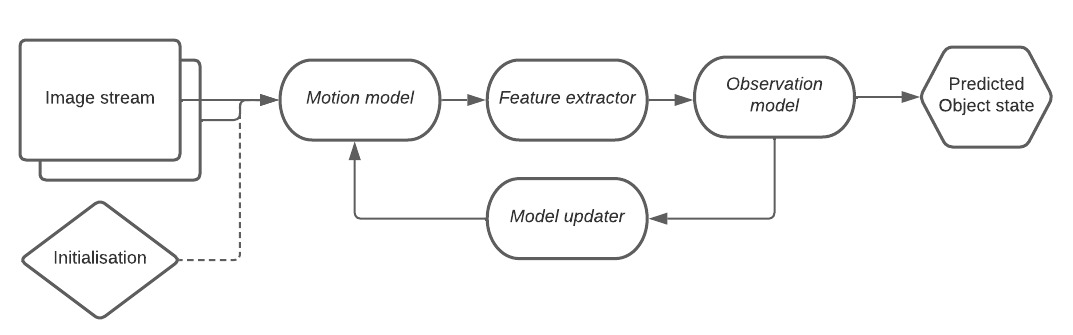
\includegraphics[width=13.5cm]{images/Tracking_flowchart.jpeg}
\caption{Generalized tracker flowchart (Redrawn from \cite{diagnosingtrack})}
\label{fig:tracker}
\end{center}
\end{figure}

\pagebreak
The components are described as follows:

\begin{itemize}
    \item Initialization -- An object to be tracked is selected manually or by detection.
    \item Motion model -- Generates candidates that may contain the tracked object.
    \item Feature extractor -- Acquires a representation of the objects in the image.
    \item Observation model -- Classify if is the tracked object. Assigns detection to target.
    \item Model Updater -- Adaptation of the observation model.
\end{itemize}

It is reported that not all components have equal importance, which is useful insight when real-time performance is desired. \cite{diagnosingtrack} conclude, \textit{``Contrary to popular belief, it turns out that the observation model (which is the focus of many papers on visual tracking) does not play the most important role in a tracker''}. Feature extraction is found to affect the performance most - which is a task that CNNs excel at. An object tracker which utilities the progress of CNN detection methods is a popular algorithm: ``Simple Online and Real-time tracking'' (SORT) \citep{sort}.

\subsection{SORT}

SORT is a visual object tracking technique which is based on the Kalman filter \citep{kalman} and Hungarian method \citep{hungarian}. A Kalman filter is a recursive state estimator which fuses a motion model and measurement to predict the motion state of a linear system \citep{trackbook}. 

\subsubsection{Kalman filtering}

In this model, object motion is described by a discrete linear time invariant (LTI) state-space process which defines the evolution of the state from time $t-1$ to time $t$ as:
\begin{equation} 
x_t=Fx_{t-1}+Bu_{t}+w_{t}
\end{equation}
Where $x_{t}$ is the object state at time $t$ of ($n \times 1$) shape, $F$ is the state transition matrix (from a system dynamics model) of ($n \times n$) shape which describes how the state evolves between time $t$ and $t-1$. $B$ is the control-input matrix and $u$ the control vector which models the effect of control signals into the system. $w$ is the process noise vector which is normally distributed about a mean of zero with process error covariance $Q$ which accounts for neglected and uncertain modeled behavior.

An observation model describes the relationship between the object state and the measurement at the current time step:
\begin{equation} 
z_t=Hx_{t}+{\upsilon}_t
\end{equation}
Where $z_{t}$ is the measurement vector at time $t$ of ($m \times 1$) shape, $H$ is the measurement matrix of ($m \times n$) shape which maps measurements to the object state. $\upsilon$ is the measurement noise vector which is normally distributed about a mean of zero with variance $R$ which accounts for measurement uncertainty.

The Kalman filtering algorithm is then performed for state estimation as follows. The ``prediction step'' is computed as:
\begin{equation}
\hat{x}_{t|t-1}=F\hat{x}_{t-1|t-1}+Bu_{t|t}
\end{equation}
\begin{equation}
\hat{P}_{t|t-1}=F\hat{P}_{t-1|t-1}F^T+Q 
\end{equation}
Where $\hat{x}_{t|t-1}$ and $\hat{P}_{t|t-1}$ are the state and the covariance predictions at  time $t$. 

The ``correction step'' is then computed as:
\begin{equation} 
K = \hat{P}_{t|t-1}H^T(H\hat{P}_{t|t-1}H^T+R)^{-1}
\end{equation}
\begin{equation} 
\hat{x}_{t|t} = \hat{x}_{t|t-1}+K(z_t-H\hat{x}_{t|t-1})
\end{equation}
\begin{equation} 
\hat{P}_{t|t}=(I-KH)\hat{P}_{t|t-1}
\end{equation}
$K$ is known as the Kalman gain which, for linear systems with gaussian noise, can be optimally computed for mean-square error to apply a correction based on the relative uncertainty between the process and measurement. This can be understood as a trade-off between the model predicted state and the measurement. In typical usage, $\hat{P}_0$ is initialized to a relatively high value which has the impact of the system favoring the measured state while the state estimate is very uncertain.

In the case of a nonlinear state transition or measurement mapping, object motion can be modeled more generally by:
\begin{equation} 
x_t=f(x_{t-1},u_{t})+w_{t}
\end{equation}
\begin{equation} 
z_t=h(x_{t})+{\upsilon}_t
\end{equation}
Systems with nonlinear state transition or measurement mappings can be linearized at each time step, using the Taylor series expansion, and used in the standard equations to obtain the Extended Kalman Filter (EKF) \citep{trackbook}. The resulting matrices can each be computed as the Jacobian matrix (first-order partial derivatives):
\begin{equation}
F_t = \frac{\partial f(\mu_{t-1}, u_{t})}{\partial x_{t-1}}
\end{equation}
\begin{equation} 
H_t = \frac{\partial h(\mu_{t})}{\partial x_t} 
\end{equation}
Here $\mu$ refers to the state about which the linearization occurs. The EKF is non-optimal however remains powerful and popularly used.

\subsubsection{SORT algorithm}

With real-time performance being a crucial component of online tracking, the light weight and minimalist nature of the SORT algorithm supports rapid update cycles. Despite its simplicity, it performs exceptionally well. \cite{sort} state, \textit{``This approach achieves an accuracy comparable to state-of-the-art online trackers.''} Furthermore, due to the computational simplicity of their method, the algorithm achieves a rapid update rate of 260 Hz which is quoted to be over 20x faster than other state-of-the-art trackers and certainly exceeding real-time requirements.

SORT comprises of the following components:
\begin{itemize}
	\item A first order Kalman filter (linear constant velocity assumption) which is used to model the states of a tracked object. Without a detection associated to the object, its state is simply predicted without correction using the linear velocity model. With an associated detection, the predicted bounding box (BB) can be used to update the object states using the Kalman filtering algorithm.

	The state of each object is modelled as:
\begin{equation}
x = [u,v,s,r,\dot{u},\dot{v},\dot{s}]^T
\end{equation}
With u and v representing the horizontal and vertical location of the center of the object and the area (s) and aspect ratio (r) of the target’s bounding box.

	\item For feature extraction, the original implementation uses an object detector known as ``Faster R-CNN'', however, since SORT utilities only bounding box position and size for both motion estimation and data association it is possible to evaluate and choose any sufficiently performing object detector \citep{sort}.
	\item To assign detections, each object's new bounding box is predicted. The IoU score (see object detection) is then computed between each detection and all predicted bounding boxes and the association problem is then solved optimally using the Hungarian algorithm.
\end{itemize}

\cite{sort} reiterate the strong influence of object detector performance on overall tracking results. Further, the relevance of the Kalman filter is reaffirmed in modern tracking applications. More recent work by \cite{sort++} shows that a constant velocity model with a Kalman filter and Hungarian method is still a powerful tracking approach. For robotics applications, \cite{sortrob} states that SORT trackers are still \textit{``achieving state-of-the-art results with a high frame rate''} 

\subsection{Deep SORT}

As an extension to the SORT algorithm, Deep SORT (Simple Online and Real-time Tracking With a Deep Association Metric) has been introduced by \cite{deepsort}. In this extension, appearance information is included into the observation model in an attempt to improve the performance for multiple objects. The addition is effective at reducing the number of identity switches, which permits longer periods of occlusions, however, it comes at a cost of real-time performance. Therefore in the case of real-time single object tracking, it does not provide sufficient benefits over SORT. 

\pagebreak
\subsection{KalmanNet}

The Kalman filter remains an effective and popular tracking algorithm which finds itself in common use in computer vision and robotics \citep{kalmanforever}. A downside of  motion model based methods is that performance relies on accurate knowledge of the underlying dynamics -- which typically requires domain knowledge and valid assumptions. Modern data driven approaches try to learn entirely from data, however, they have many parameters, require significant amounts of data and lack intuition, which ultimately prevents their application in embedded systems \citep{kalmannet}.

\cite{kalmannet} propose a hybrid data-driven and model based approach to real-time Kalman filtering, where the underlying state space model is non-linear and accurate knowledge of it is unknown. In this approach a recurrent neural network (RNN) (more specifically a Gated Recurrent Unit (GRU) variant) is trained on representative data in order to predict the appropriate Kalman gain at each time step  (See figure \ref{fig:blockd}). Compared to ``traditional'' feed-forward neural networks where fixed length input data simply flows through the network to compute an output, in an RNN the input as well as a hidden state (which represents the history) are fed back into the network -- which allows a series of temporal information to be processed  (See figure \ref{fig:architecture}). 

\begin{figure}[h!]
\begin{center}
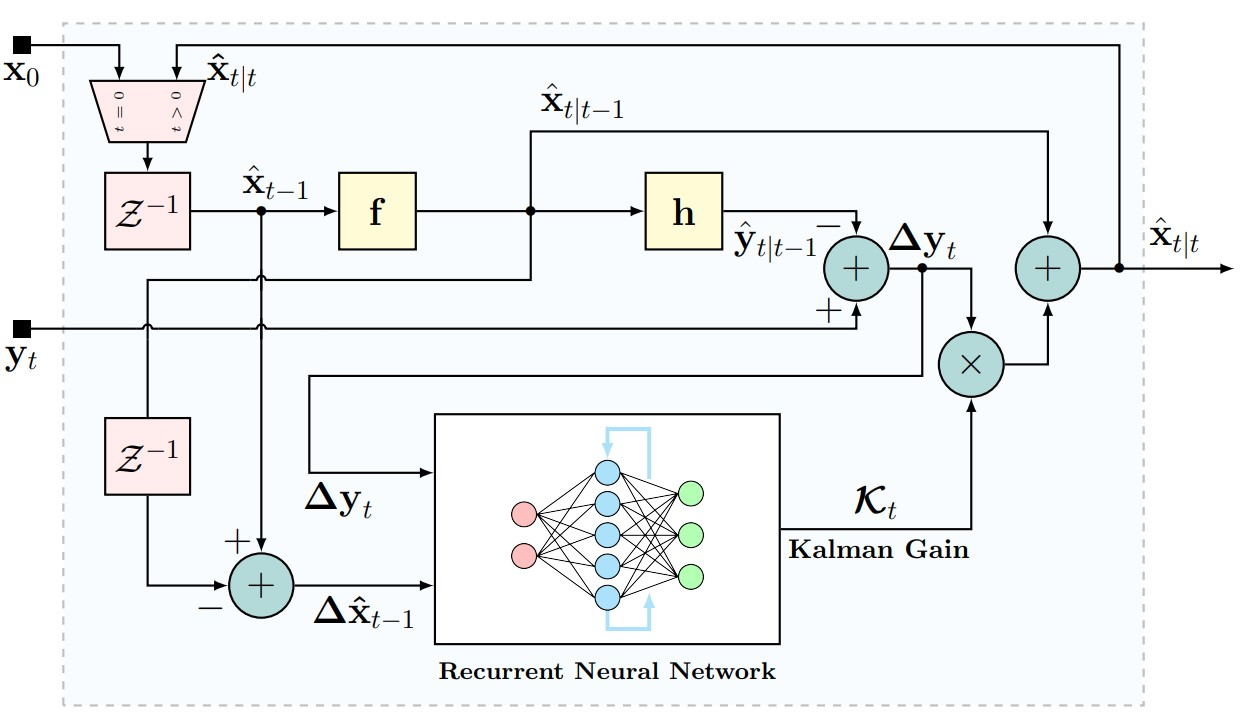
\includegraphics[width=12.5cm]{images/kalmannet1.jpg}
\caption{KalmanNet block diagram \citep{kalmannet}}
\label{fig:blockd}
\end{center}
\end{figure}

\begin{figure}[h!]
\begin{center}
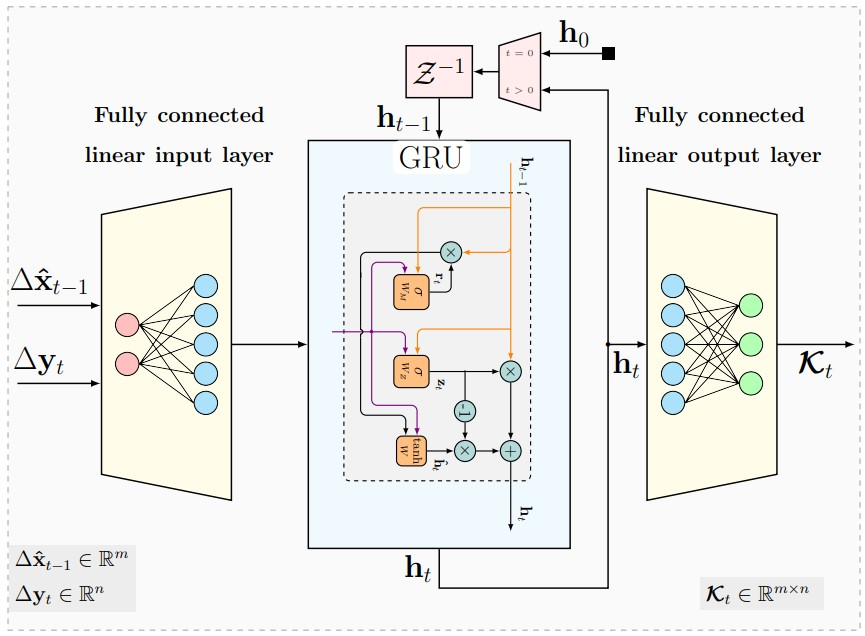
\includegraphics[width=10cm]{images/kalmannet2.jpg}
\caption{KalmanNet RNN \citep{kalmannet}}
\label{fig:architecture}
\end{center}
\end{figure}

In this manner, KalmanNet aims to remove the dependency of accurate knowledge of the underlying process and measurement noise and a facilitates a partially known or approximated underlying state space model from a system dynamics model. The model can be trained end-to-end which means that the Kalman filter is embedded in the network and a loss function can be formulated to evaluate the tracking performance directly, rather than by training intermediate subcomponents and creating a pipeline.

The interpretability of the original algorithm can be retained whilst potentially learning complex dynamics implicitly, reducing the need for domain knowledge and model assumptions that are needed to accurately characterize a complex system as a tractable state space model. \cite{kalmannet} conclude, \textit{``KalmanNet is shown to converge much faster compared with purely data driven systems, while outperforming the model based extended Kalman filter, Unscented Kalman filter and particle filter, when facing model mismatch and dominant non-linearities''}. This data driven approach to Kalman filtering has recently found other robotics applications -- replacing the extended Kalman filter for online Simultaneous localization and mapping (SLAM) -- a crucial task for robotic systems where a map of an environment is simultaneously constructed while localizing the position of an agent \citep{slam}.

\subsection{Performance measures}

A useful performance measure used for evaluating state estimators is the Root Mean Square Error (RMSE) -- which can be considered as the standard deviation of the difference between the predicted state and the ground truth. \citep{kalmanperform}

RMSE can be computed as follows:
\begin{equation}
RMSE = \sqrt{\frac{1}{M}\sum^{M}_{i=1}\epsilon_{i}^{2}}
\end{equation}

Where $\epsilon_{i}$ is the error for the $i$th sample which is difference between the predicted and ground truth state. RMSE is often used as a statistical design criterion for noisy systems as it prescribes a soft bounds based on probability (for true Gaussian noise it is by definition that 99.7\% of samples will occur within three standard deviations).

\newpage
\section{Object detection}

Object detection is one of the oldest and most fundamental computer vision problems. Within the scope of this problem is facial recognition, pedestrian recognition and multi-class classification which have historically received significant attention in various competitions and the establishment of various  datasets such as Caltech pedestrians \citep{peddetect}, PascalVOC \citep{vocdataset} and Microsoft COCO \citep{coco}.

\subsection{Traditional Object detection}

With the most successful approaches being based on discriminative models -- a traditional object detector can be considered in general to have the following components:  Region selection, feature extraction and classification \citep{deepreview}:

\begin{itemize}
    \item In region selection, different sub windows are considered at various scales and are passed into the detector window. This may be by a region proposal algorithm or by scanning the entire image at different scales. This approach is less intensive than processing the entire image in a single pass and allows a single detector to be trained and applied throughout the image, but is computationally expensive. 
    \item Feature extraction attempts to capture patterns in the image that represent an object or provide semantic information. Low level features (textures, edges, etc.) may be combined with spacial information into a single feature descriptor.
    \item A classifier predicts the presence of an object class in the window given the extracted features. The decision boundary (which is an $n-1$ dimensional surface in an $n$ dimensional domain) is learnt using training examples. For a positive detection, the current window is returned as a bounding box. Since multiple windows will return positive for the same object, techniques such as non maximum suppression can be used to isolate a single prediction.
\end{itemize}

\noindent Some of the criticisms of traditional strategies are: 
\begin{itemize}
    \setlength\itemsep{0em}
    \item Generating bounding boxes with a sliding window strategy is inefficient and the localization is often inaccurate (loose fitting bounding boxes).
    \item Using hand crafted low level features it is difficult to adequately capture the semantics of the image 
\end{itemize}

Traditional object detectors that had relative success and some real-time application include the Viola Jones algorithm \citep{vjdet} as well as the HOG features and SVM classification based D\&T detector \citep{hog}. 

\subsubsection{Viola Jones detection}

The Viola Jones (VJ) detector \cite{vjdet} was a breakthrough algorithm that was considered to be the first viable real-time object detector still maintaining state-of-the-art accuracy. Although targeting face detection, it can be equally applied to different object classes. The VJ detector uses a sliding window detector with a fixed step size. A scaling factor can be applied to the window which increases the filter size proportionally after each complete image traversal in order to search for larger faces. 

Firstly considering feature extraction, an observation can be made that classes of objects, such as faces, have a typical layout that can be approximated by patterns of adjacent lighter and darker regions. These ``Haar-like'' features (Figure \ref{fig:haarft}) are applied to a gray-scale image to capture the differences in regions with a single number. Filters of pattern A and B respond to edges, filters of pattern C respond to lines and filters of pattern D respond to diagonal features. During training, an exhaustive search for features is performed where all possible scale, aspect ratios and positions of the filters in the detection window are considered for each training face example - in the case of a 24x24 window approximately 180k features exist each detection window. 

\begin{figure}[h!]
    \centering
    \subfloat{{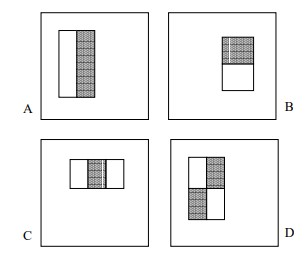
\includegraphics[height=5cm]{images/haarft.jpg}}\label{fig:haarft}}
    \qquad
    \subfloat{{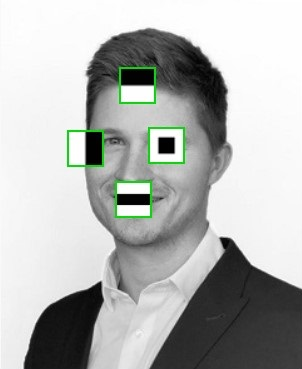
\includegraphics[height=5cm]{images/vjtest.jpg}}}
    \caption{Haar features \cite{vjdet} (Left) and strong responses (Right)}
\end{figure}

\citeauthor{vjdet} (\citeyear{vjdet}) introduce an elegant approach to evaluate these features rapidly by precomputing an intermediate ``integral image'' which allows the subsequent computation of a region in constant time as it only has to be evaluated once per image and can then be used for each feature.

In order to classify each window, there are a significant number of Haar-like features possible at each possible detection. An efficient approach to classification, based on the adaBoost machine learning algorithm, is used as a ``feature selection'' process by training and selecting a subset of weak classifiers that can be combined into a strong classifier. The set of ``cascading classifiers'' are arranged as a degenerate decision tree, where each node is a stage of increasing complexity. Negative classifications cause an early exit from the cascade, therefore background regions are usually rejected quickly and more computation is spent on distinguishing complex regions.  Multiple stages may be used, which are progressively more ``difficult'' to pass - candidates which pass all stages in the
cascade are classified as the target object.

The speed of processing an image is therefore impacted by the complexity of the image (complex backgrounds can slow it down). Using less stages and features can result in faster compute times. Faster speeds can also be achieved by increasing the step sizes and scaling factor. Models which are under-trained tend to focus on background areas which can lead to impracticable inference times. 

\newpage
\subsection{Modern Object detection}

Before the dramatic growth and change of focus towards modern computer vision techniques, traditional object detectors were reaching saturation. \cite{rcnn} writes: \textit{``Object detection performance, as measured on the canonical PASCAL VOC dataset, has plateaued in the last few years. The best-performing methods are complex ensemble systems that typically combine multiple low-level image features with high-level context''}.

Deep learning approaches are considered to have become the state of the art since the year 2012 with AlexNet becoming the first CNN to lead the ImageNet Large Scale Visual Recognition Challenge (ILSVRC) \citep{alexnet}. The first widely popularized object detector to make use of CNNs is R-CNN (Regions with CNN features) \citep{rcnn}, which uses CNNs for feature extraction but otherwise retains a traditional detector pipeline with region proposal. CNN based detectors which utilize a region proposal stage and are known as two-stage detectors \citep{comprehensive}.  Modern object detectors are able to achieve near perfect results on datasets that traditional architectures fail to show even marginal comprehension of. This can be seen in the benchmarking of the You Only Look Once (YOLO) object detector (See figure \ref{fig:yoloplot}) \citep{yolo} versus the famous ``D\&T'' detector of \cite{hog}.

\begin{figure}[h!]
\begin{center}
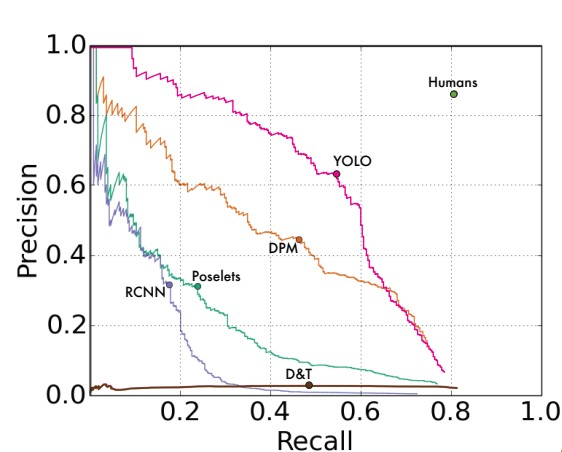
\includegraphics[width=8.5cm]{images/yoloplot.jpg}
\caption{YOLO precision-recall curve \citep{yolo}}
\label{fig:yoloplot}
\end{center}
\end{figure}

Modern object detectors utilize deep CNNs in order to learn feature extraction. CNNs are based upon the mathematical operation of convolution, where a matrix of trainable weights called a filter kernel is swept across an image. CNNs take advantage of the spacial context of an image and are able to extract both low level and high level contextual features due to a hierarchical network structure, often referred to as the backbone of the network. The networks can be trained by minimizing a loss function that combines the regression and classification performances by using an algorithm known as back propagation to search for optimum kernel weights. The object detection problem can be considered as the combination of both classification and regression tasks. A loss function is a measure of the error of the prediction for the considered task and the aim of training is to find a local minimum of this objective.

Least square error ($L_2$ loss) is a common choice for regression loss when considering continuous variables:
\begin{equation}
L_{regression} = \sum(y_i-\hat{y_i})^2 
\end{equation} 
Where $y_i$ is the ground truth.

Categorical cross-entropy loss is a popular choice for classification tasks, when categorical variables are considered, as it is readily differentiable for back-propagation:
\begin{equation}
L_{classification} = -\sum_{i=1}^{n}t_i log(p_i)
\end{equation} 
With $t_i$ being the ground-truth and $p_i$ being the softmax probability for the $i_{th}$ class.

More recent architectures have seen great success by encouraging models to learn from more challenging examples, rather than focusing on ``easy'' examples, by adding an additional factor which reduces the weighting of easy cases. Such a loss function is known as a ``focal loss''. \citep{focal}
\begin{equation}
L_{focal} = -\sum_{i=1}^{n} (1-p_i)^\gamma log(p_i)
\end{equation} 
Where $\gamma$ is a tune-able variable known as the focusing parameter.

Various loss functions can be combined into a multipart loss function which is engineered to achieve a certain behavior.

\subsubsection{YOLO}

A breakthrough for real-time object detection was achieved with the introduction of the one-stage (AKA single-shot) detector YOLO by \cite{yolo} which achieved real-time speeds whilst remaining competitive with state-of-the-art detectors. The speed of single stage detectors is in general considered to be faster than that of two-stage detectors -- but at a cost of accuracy. According to \cite{stagecomp} regarding two stage detection: \textit{``This architecture can achieve more reliable detection, but increases the required computation, hence being less convenient for real-time applications''}. 

\begin{figure}[h!]
\begin{center}
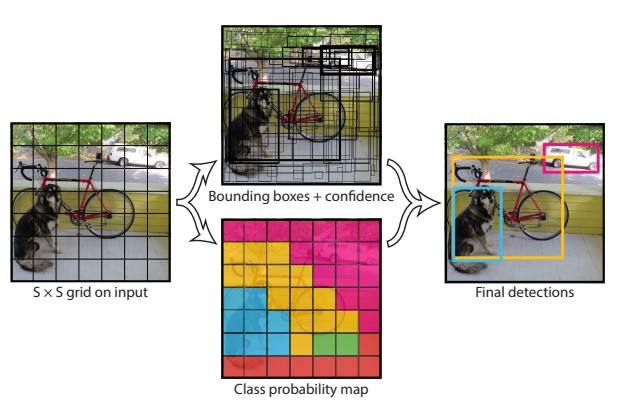
\includegraphics[width=7.5cm]{images/yolodemo.jpg}
\caption{YOLO object detection \citep{yolo}}
\label{fig:yolodemo}
\end{center}
\end{figure}

In the basic YOLO architecture by \cite{yolo}, the image is divided into an $S \times S$ grid. Each grid cell is used to predict $B$ bounding boxes with associated confidence scores and $C$ class probabilities which is demonstrated in figure \ref{fig:yolodemo}. This is done by passing the output of the backbone into fully connected layers with output nodes representing each cell. \cite{yolo} considers disadvantages of this approach to be a sensitivity to hyper-parameters, difficulty detecting objects much smaller than the anchors as well as suffering localization error: \textit{``While it can quickly identify objects in images it struggles to precisely localize some objects, especially small ones''}. 

To achieve additional performance, the YOLOv2 architecture by \cite{yolov2} introduces (besides other incremental improvements) the usage of predefined bounding boxes which are used as initial guesses to facilitate the model learning more diverse object sizes and aspect ratios. These are known as ``anchor'' boxes, with the technique dubbed an anchor-based approach. The box dimensions (dimensional priors) are learnt by k-means clustering of the dataset. Further improvements have been made with YOLOv3 \citep{yolov3} and YOLOv4 \citep{yolov4}, with the most significant enhancements being a deeper and more optimized backbone, a loss function tailored to the evaluation metric as well including various proven pre and post-processing tricks (``bag-of-freebies and ``bag-of-specials'') to improve the accuracy with little overhead. These models are also released with a ``tiny'' version which further trades accuracy for speed and model size. Note that numerous unofficial ``YOLO'' detectors have also been created which have no affiliation to the original researchers.

\subsubsection{NanoDet}

Contemporary object detection advancements include anchor box free detectors -- by reformulating the problem as ``keypoint'' detection. \cite{comprehensive} report: \textit{``The keypoint-based methods generally outperform the anchor-based and two-stage methods in terms of accuracy and speed''}. Although CornerNet \citep{cornernet} was proposed as the first alternative to the single stage anchor-based approaches, more recent and successful models include Fully Convolutional One-stage Object Detection (FCOS) \citep{fcos} and the subsequent NanoDet \citep{nanodet} which has been shown to be the current state-of-the-art for real-time object detection as demonstrated by the comprehensive study of \cite{comprehensive}.

\begin{figure}[h!]
\begin{center}
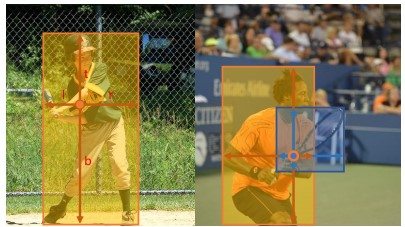
\includegraphics[width=9cm]{images/keypointdetect.jpg}
\caption{Keypoint based object detection \citep{fcos}}
\label{fig:keypointdetect}
\end{center}
\end{figure}

In the ``FCOS-style'' key-point approach which NanoDet is based on, each object is modeled as a single center point of a bounding box. The network is used to predict heatmaps where the intensity peaks are representing keypoints. Regression of the bounding boxes can then be performed utilizing key-points rather than anchors. A benefit of this approach is that it eliminates the anchor-box hyper-parameters, which are dataset-dependant, as well as avoiding the problem of having to compute and reject redundant (non-maximal) box predictions. According to \cite{cnet} \textit{``Most successful object detectors enumerate a nearly exhaustive list of potential object locations and classify each. This is wasteful, inefficient, and requires additional post-processing.''}   

After passing the input image through the convolutional backbone for feature extraction, NanoDet utilizes a modified lightweight Path Aggregation network (PAN) \citep{pan, nanodet} neck before passing the output to it's detection head. PAN is an incremental improvement of a Feature Pyramid Network \citep{fpn} which is a popular technique in the object detection space. In a feature pyramid network, the output feature maps taken from various shallow and deeper levels from the backbone network (representing spacial and semantic information respectively) are utilized by the model to better detect objects across a range of scales. This is a similar concept to the idea of an image pyramid which is popular with traditional approaches, however it naturally leverages the pyramidal hierarchy of the backbone without the additional computational overhead.

\subsection{Performance Measures}

In order to evaluate object detection algorithms, it is important to choose a measure that represents the desired performance in a comparable manner (not algorithm specific). In the context of classification, a tempting approach is to evaluate the accuracy:
\begin{equation}
Accuracy = \frac{TP + TN}{TP + FP + TN + FN}
\end{equation}
However, in the case of class imbalance this measure gives misleading results. Consider an extreme of 0.5\% of ground truth labels being positive in a dataset -- a classifier that predicts all labels as negative will achieve 99.5\% accuracy, however will not have learnt any aspect of the data. Therefore precision is often used, which considers the correctness of the positive predictions that have been made:
\begin{equation}
Precision = \frac{TP}{TP + FP}
\end{equation}
This metric however only considers the cases when a prediction has been made. Therefore it must be considered with along with recall (sensitivity) which considers what proportion has been successfully predicted across the entire dataset:
\begin{equation}
Recall = \frac{TP}{TP + FN}
\end{equation}
In the extreme of using only recall, all examples can be classified positive and no learning will have occurred. Therefore precision and recall must be considered together.

Precision and recall have a relationship (See fig \ref{fig:yoloplot}) through the chosen threshold of the confidence value, as only making predictions when the confidence is high, means that less confident cases will be missed. The relationship can be plotted as an ROC curve, however, comparing the performance of multiple algorithms using this approach makes it difficult to evaluate quantitatively. In order to represent this curve as a single value for comparison, there are a variety of approaches possible including F1 score, Area Under Curve and Average Precision (AP).

AP is a popular metric used in the context of modern object detection -- traditionally calculated by averaging the sum of the precisions $p$ across 11 evenly distributed levels in recall. A good score requires high precision and recall $r$: \citep{vocdataset}.

\begin{equation}
AP = \frac{1}{11}\sum_{r\in\left\{0,0.1,0.2,...,1\right\}}^{} p_{interp}(r)
\end{equation}
where:
\begin{equation}
p_{interp}(r) =\max_{\widetilde{r} > r} p(\widetilde{r})
\end{equation}

$AP_{small}$, $AP_{medium}$, $AP_{large}$ are variations used to denote differently sized detection objects (COCO consider images less than $32 \times 32$ as small and larger than $64 \times 64$ as large), to get an understanding of the performance over scale. In order to account for multiple classes, the mean average precision (mAP) is commonly computed which is nothing but the sum of the AP per class divided by the number of classes:

\begin{equation}
mAP = \frac{1}{N}\sum_{i=1}^{N} AP_{i}
\end{equation}

When detecting an object, a bounding box is placed around the target. It is possible to compare quality of the localization prediction with the ground truth by evaluating the overlapping areas -- called Intersection-over-union (IoU). A perfect overlap results in a score of 1 and a score of 0 for a complete miss. AP may be evaluated at a given threshold of IOU, for example an IoU of 0.5 may be specified (denoted as AP@.50). A series of IoU might be used by averaging the AP results over the range to try evaluate the results in isolation of threshold (denoted as AP@[.5 : .95]).  \citep{pmetrics}

A criticism of these commonly used metrics is that they do not consider run-time or memory usage -- which are required for practical deployment. The real-time performance is difficult to compare between algorithms since most papers do not go into significant depth regarding the relationship between accuracy and speed \citep{speedacc} -- with most vision applications focusing on quality of prediction. A further challenge is that the actual real-time performance is also largely dependent on the hardware and software infrastructure on which the algorithm is executed. An approach to understanding the run-time performance (sometimes called latency) of different architectures is to consider relative comparisons that are bench-marked under the same conditions. Typical metrics are frames per second (FPS) or Hz.

\newpage
\subsection{Optimizing models for real-time performance}

In practice, a trade off exists between the real-time performance and accuracy achieved by a model when performing inference. Intuitively, when less data is taken into consideration -- such as by the reduction of image resolution -- inference can be faster as it requires less computation, however, the accuracy may decrease as the detail and structure of the data is lost. Therefore the performance of a computer vision algorithm should not be evaluated in isolation of latency for real-time application. According to \cite{speedacc}, many computer vision architectures tend to focus on accuracy and therefore may use model ensembling and multicrop methods which are too slow for practical real-time implementation.

Deep learning models in particular tend to be large in both memory and computational demands relative to the capacity of typically spatially and power constrained embedded robotics computers. \cite{quantization} write, \textit{``This creates a problem for realizing pervasive deep learning, which requires real-time inference, with low energy consumption and high accuracy, in resource-constrained environments''}. Apart from selecting efficient network architectures, quantization offers possible means to reduce memory consumption and computational costs of a model which can result in improved real-time performance. The aim of quantization is to represent the weights and activations of the model with reduced precision without a significant impact on accuracy. 

\subsection{Neural Network development and deployment}

A variety of software tools have been developed in order to abstract the low level implementation details of neural networks from high level model architecture for the convenience of the researcher. New deep learning frameworks have often coincided with leaps in network performance such as Caffe (Berkeley AI) \citep{caffe} utilised for the development of R-CNN \citep{rcnn} as well as Darknet used for the development of YOLO \citep{yolo}. Popular contemporary frameworks such as Tensor Flow (Google) \citep{tensorflow} and Pytorch (Facebook) \citep{pytorch} facilitate the development of a variety of deep learning model architectures such as CNN, RNN, and fully connected networks as well as providing support for CPU and GPU accelerated training and inference. These frameworks are meticulously maintained, continuously developed in an open source community and have the vast resources of tech giants which supports the current rapid growth of machine learning technologies.

Researchers often implement model architectures using the paradigm of a particular framework and therefore models are often not easily interchangeable between frameworks. Further, the libraries and tooling provided by these frameworks are typically used in the context of development and training therefore are therefore not optimum environments for practical model deployment where only the forward pass is desired as they are large in memory are not necessarily portable between computing architecture and platform. In the context of a real world multidisciplinary development environment with many interacting components, such as in Robotics, it is good practice to consider the management of subsystems, the run-time environment as well as avoiding a framework dependency so that models from a variety of frameworks might be used. 

Although some popular computer vision packages such as OpenCV do have an interface to load models from a limited set of frameworks -- not all operations are supported, each framework has different configurations and run-time optimization is not possible, Empirically, the real-time performance is poor. Open Neural Network Exchange (ONNX) is a well accepted standard \citep{onnx} for machine learning interoperability that provides a neutral format which can be executed in the ONNX Runtime environment (Microsoft). This inference engine supports different neural network types, multiple platforms, hardware architectures, operations as well as execution and model optimizations such as quantitation. Models compiled to be run on ONNX Runtime have shown to receive significant real-time performance improvements \citep{inference}.

\begin{figure}[h!]
\begin{center}
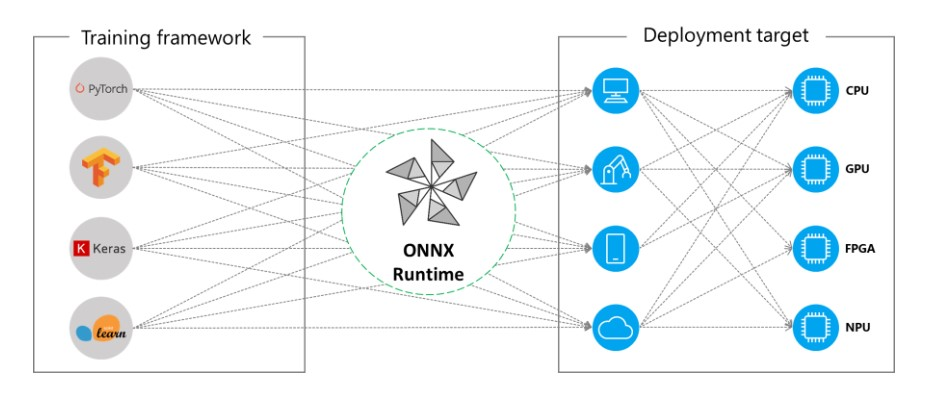
\includegraphics[width=10.5cm]{images/onnx.jpg}
\caption{ONNX Model environments \citep{onnx}}
\label{fig:onnxplot}
\end{center}
\end{figure}

\section{RoboCup Soccer}
RoboCup is an internationally coordinated robotics competition with a focus on advancing artificial intelligence and robotics research. The ultimate goal of the soccer competition is to support the development of a team of fully autonomous humanoid robot soccer players that are capable of winning against the winner of the most recent soccer world cup, by the year 2050. The RoboCup challenge features a dynamic environment and distributed control performed in real-time \citep{RoboCupObj}.\

There are various leagues which each emphasize different challenges that need to be addressed to achieve the ultimate RoboCup objective. Of particular interest is the RoboCup 3D Soccer Simulation League (3DSSL) -- which is demonstated in figures \ref{fig:robofb} and \ref{fig:agentview} -- as well as the Standard Platform League (SPL), which focuses on the software programming aspects of Nao robots. The Nao v5 features an Intel Atom Z530 CPU with 1GB RAM \citep{naov5}.

\begin{figure}[h!]
\begin{center}
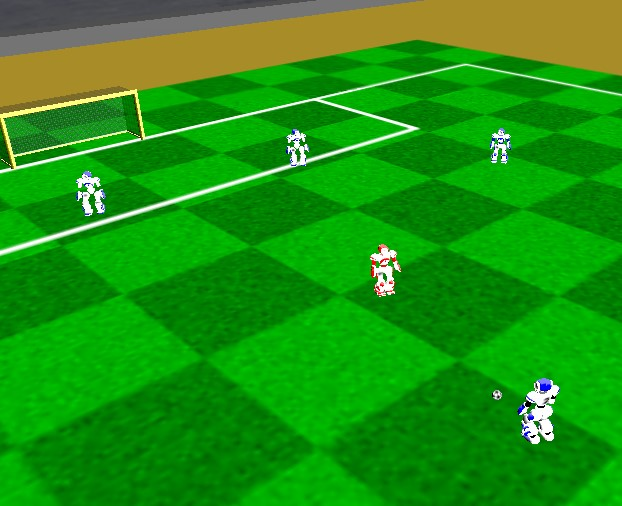
\includegraphics[width=9.5cm]{images/Robocup1.jpg}
\caption{Simulated RoboCup Soccer}
\label{fig:robofb}
\end{center}
\end{figure}

\begin{figure}[h!]
\begin{center}
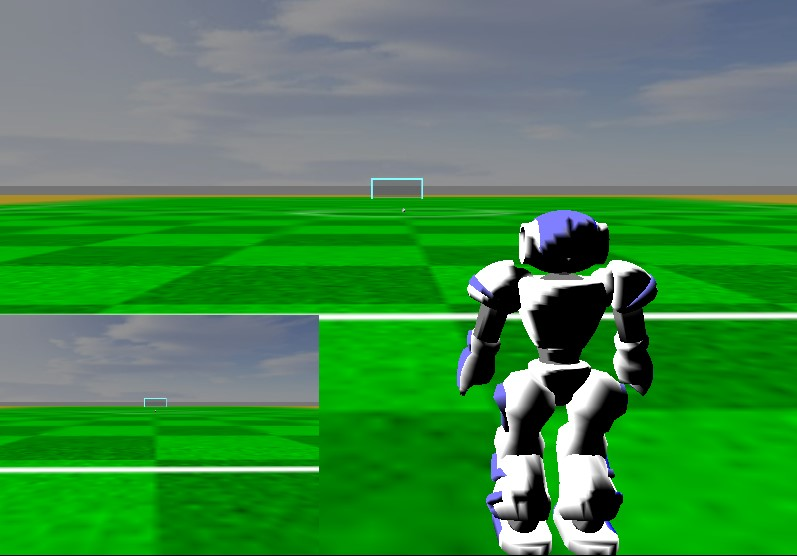
\includegraphics[width=9.5cm]{images/Robocup2.jpg}
\caption{Simulated image perceptor (Agent perspective in subwindow with a ball in the distance)}
\label{fig:agentview}
\end{center}
\end{figure}

The position of the ball is crucial for determining appropriate agent behavior. At a close observation range the agent may need to kick the ball, in this case large errors will result in a miss-directed kick or perhaps a complete miss. At middle ranges the agent may attempt to block an opposition passing option and should position itself accordingly. At long ranges the agent may need to know what region of the field the ball is in so that an appropriate behavior is chosen. 

\subsection{RoboCup Soccer Simulator}

The RoboCup 3D Soccer Simulation League runs on a simulator known as the RoboCup Soccer Simulator Server (RCSSServer3d) which is developed using plugins to a generic physical multi-agent simulation platform, SimSpark. In the architecture of SimSpark, agents receive various sensor feedback from ``perceptors'' and take actions using ``effectors'' \citep{simspark}. In the current format of 3DSSL, a vision perceptor returns prepossessed visual data, in spherical coordinates, to each agent every two simulation cycles (40ms). Therefore in this league, computer vision is not within the scope of the challenge. The capabilities do however exist within the underlying SimSpark simulator to provide an image perceptor that produces rendered simulated camera images by enabling a plugin.

%\subsection{Nao}
%The Aldebaran Nao robot is the agent used in the 3DSSL and SPL RoboCup leagues. The robot has two cameras (figure \ref{fig:naocam}) placed on the head which can be rotated by a joint effector on the neck of the Nao (figure \ref{fig:naoneck}) to scan across the field. In the physical robot, the output image is given in a YUV colour space captured in 1280x960 at 30fps -- However it is possible to reduce the resolution of the camera and capture rate
%\citep{aldebaran}.
%
%\begin{figure}[h!]
%    \centering
%    \subfloat{{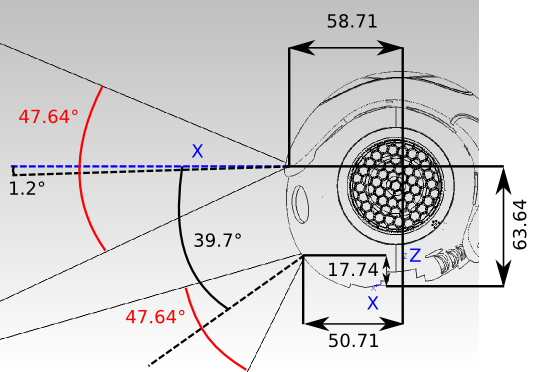
\includegraphics[height=4cm]{images/nao1.png}}}%
%    \subfloat{{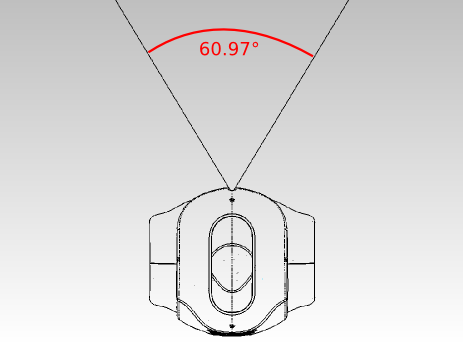
\includegraphics[height=4cm]{images/nao2.png}}}%
%    \caption{Nao Camera configuration \citep{aldebaran}}
%    \label{fig:naocam}
%\end{figure}
%
%\begin{figure}[h!]
%	\begin{center}
%	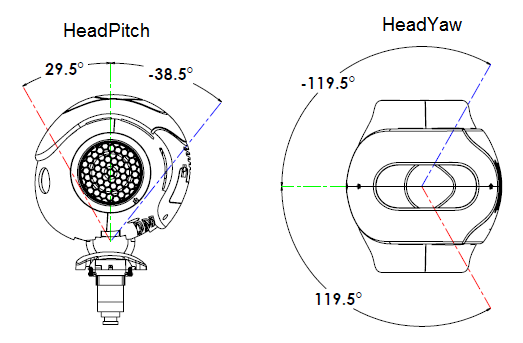
\includegraphics[width=7cm]{images/nao3.png}
%	\caption{Nao Neck effector \citep{aldebaran}}
%	\label{fig:naoneck}
%	\end{center}
%\end{figure}
%
%With the given camera configuration, the Nao has monocular vision. Further, due to the limited FOV of the cameras as well as the range limited yaw rotation of the Nao neck effector, there is a blind spot behind the robot. The two cameras can be accessed simultaneously. The Nao v6 features an intel Atom E3845 1.91Ghz Quad core CPU with 4GB DDR3 RAM \citep{naov6}.
%
%\subsection{Fat Proxy}
%Fat proxy is a sub league of the RoboCup Soccer simulation league which focuses on high level behavior by providing a common set of low level skills such as walking and kicking. The developers \cite{fatproxy} state, \textit{``To have simplified access to the simspark simulation, the Fat Proxy takes over all motor control of the simulated Nao robots. Agents control the robot with high level dash and kick commands. Anything else like getting up or focusing the head is done by the Fat Proxy''}. The tooling for this is useful as it can be used to isolate higher level behaviors from the low level skills of the robot.

\chapter{Related work}

In this section, a selection of published works that are related to ball detection  (Section 3.1) and tracking (Section 3.2) in RoboCup are considered. This overview lists some important approaches and results whilst keeping in mind the historical context of traditional versus modern techniques by arranging them chronologically. It is shown that recent approaches take advantage of fine tuning state-of-the-art CNN object detector architectures for transferring to their own problem domain as well as Kalman filtering for tracking.

\section{Ball detection}

The object detection space has significantly changed over time, with the most successful detectors being deep learning based. Using what is now considered a traditional approach, \cite{robovj} implement a Viola Jones based object detector that performs real-time ball detection with a focus on mobile robots in a Robocup soccer environment. They perform a edge detection proprocessing step which allows them to achieve a satisfactory color-independent result.

Attempting to apply more modern deep learning techniques to improve real-time ball localization, \cite{selfcnn} propose a novel CNN to localize multicolored, patterned balls for Robocup by formulating their approach as a regression problem. They develop an architecture that can process an entire image at once to avoid a sliding window approach by predicting Gaussians that correspond to probabilities of the ball location. They find their proposed model to be too large for their robot (over 2GB) but also find that reducing their model size leads to a poor performance. \cite{selfcnn} conclude, \textit{``Thus, either faster processors for robots are necessary (to run the bigger nets) or low classification rates at medium to high distances have to be accepted''}. Although the design was not successful, the single shot strategy is for real-time is widely adopted by state-of-the-art detectors such as YOLO. This might also be seen as a step towards the keypoint based approach.

Basing their work on the state-of-the-art single shot architecture, YOLO v3 Tiny, \cite{robo} propose a real-time object detector which is fine tuned for RoboCup ball detection for the Nao v5 platform. The maximum reported speed is only 13 FPS. Synthetic transfer learning is successfully applied, which involves pretraining the network on a fully synthetic dataset. 

\cite{robocupdataset} evaluate several CNN models on an embedded RoboCup robotic system. They find that, for their RoboCup dataset, YOLO v4 Tiny performs the best in terms of the AP@75 metric, as well as for the small and medium images, which points towards this model being the best for accurate ball detection. However, the detector fails to execute at real-time speed on their Small Size League (SSL) platform, hence, the selection of the Mobile SSD architecture which does compute in real-time.

\section{Ball tracking}

In the ball tracking problem space, Kalman filtering has been successful and remains particularly popular. The approach of fusing measurements with a dynamic physics model allows noise attenuation as well as substep estimation for problems such as a parabolic trajectory or rolling with friction.

After winning the RoboCup-97 small-robot competition, \cite{kalmanmodel} describe their development of an EKF model -- for their team CMUnited -- to track motion of a kicked ball. The tracker includes a velocity discounting factor in the state model which is used to represent a non-linear rolling friction. 

In order to establish the real-time capability of a non-linear Kalman filtering approach for use in RoboCup, \cite{robocuptrack} investigate tracking of ball trajectories using an unscented Kalman filter (UKF) and monocular vision. Although only the tracking problem is considered (manually processed images) the investigation confirms that, compared to a maximum likelihood estimator, UKF is feasible as a real-time tracker: \textit{``after half the time of flight the error is about 0.3m which we judge to be enough for playing soccer''}.

With a focus on RoboCup Middle Size League, \cite{3dparabola} consider the use of a extended Kalman filter (EKF) for real-time 3D Ball trajectory estimation using a single camera. In their research they propose applying a maximum Likelihood method to provide an initial estimate of the ball trajectory for the initialization which improves tracking of the ball.

\cite{golftrack} investigates real-time golf ball tracking by taking advantage of state-of-the-art CNN based object detection and Kalman filter based tracking -- with small object detection as a primary focus. They report: \textit{``most object detectors do not perform well on small object detection''} where is is explained that since most detectors are pretrained on datasets, such as MS COCO, where the size of the objects tend to be larger. The detectors: Faster R-CNN, SSD, YOLO v3, YOLO v4 as well as RefineDet are investigated, however, GPU compute is available. 

%%%%%%%%%%%%%%%%%%%%%%%%%%%%%%%%%%%%%%%%%%%%%%%%%%%%%%%%%%%%%%%%%%%%%%%%%%%%%%%%%%%%%%%%%%%%%%%%
\chapter{Problem Statement, Research Aims and Objectives}
\section{Problem Statement}

In RoboCup soccer most of the decision-making involves the position of the ball on the field. This affects factors such as how the players should move, when and where they should kick and how the they should behave. In order to facilitate decision making, it is important to have an accurate understanding of the ball’s position. In this research project, the interest lies in determining if it is feasible to accurately capture the trajectory of a kicked ball in the RoboCup simulator using a computer vision based system, with a neural network based approach utilized for real-time tracking.

\section{Research Hypothesis}

Hybrid approaches to state estimation which fuse intuitive model based approaches with measured data are a promising technique for state estimation. It is hypothesized that a neural network assisted approach to Kalman filtering can outperform the traditional EKF method at tracking the trajectories of a kicked RoboCup soccer ball as measured by RMSE at real-time, using a tracking-by-detection framework.

Modern object detection has significantly improved upon traditional approaches, with contemporary models promising state-of-the-art detection with real-time performance. Tracking-by-detection is a paradigm which takes advantage of this technological leap and can be paired with the popular Kalman filter for real-time robotics applications. It is hypothesized that a more recent key-point based modern object detection approach (NanoDet) can be to used to outperform established RoboCup approaches such as an anchor based method (Yolo v4 Tiny) as well as the traditional Viola Jones detector for color-independent ball detection -- measured by quality of inference using AP scores, at a real-time speed. 

\section{Research Aims and Questions}

The first aim of the research project will be to prepare a suitable real-time object detector trained on localizing the ball in a simulated Robocup soccer environment. A traditional architecture (Viola Jones detector) alongside a more modern anchor based detector (YOLO v4 Tiny) serve as a benchmark against a recent keypoint based approach (NanoDet). To motivate the selection of NanoDet, a selection of different pretrained CNN detector models which use different strategies such as single stage, anchor-based and key-point based approaches will be compared on inference speed and memory usage. Inference speed is evaluated on a laptop CPU, acting as a compute constrained device that one might find on a mobile robotic platform. 

A significant challenge for object detection is the size of the ball which at distance is small in the image (as defined by COCO metrics). The ball used in RoboCup is also significantly white in colour and may be difficult to distinguish against the field markings, goals and Nao robots. The algorithm further needs to act in real-time since slow responses due to heavy computational load can result in delayed agent responses or leading to control inaccuracies and instability. The memory footprint of the architecture should also be considered in the context of embedded computing capacities, which can be improved using model quantization.

The principle questions which arise are:
\begin{itemize}
    \item Can an established modern CNN object detector run at real-time on a modern mobile laptop CPU?
    \item Does the more recent keypoint based NanoDet detector outperform the established RoboCup anchor based Yolo v4 Tiny and traditional Viola Jones detectors, as measured by AP in real-time on a RoboCup ball detection dataset? 
    \item Can pretraining on real images transfer to a simulated RoboCup environment?
    \item Can model quantization offer a worthwhile optimization versus performance degradation? 
\end{itemize}

The second aim of the research project will be to use the object detector to implement a tracking-by-detection framework based on neural aided Kalman filtering. Using ball telemetry from the robocup simulation as a ground truth and processing the associated visualization with the object detector, a tracker based on the KalmanNet approach can be trained. As a baseline, an extended Kalman filter can be implemented in a similar fashion to the Robocup trackers found in the related works. 

A significant challenge is the non-linearity of the trajectories due to rolling friction of the ball as well as the bouncing after the initial parabolic trajectory makes contact with the pitch. Such physics are not simply modeled in a standard linear Kalman filter. 

The principle questions which arise are:
\begin{itemize}
    \item In the context of the simulated RoboCup soccer environment, can a neural aided Kalman filter outperform a traditional EKF for tracking rolling and lofted kicks?
	\item Can a tracking-by-detection approach meet the real-time performance requirements?
\end{itemize}

%%%%%%%%%%%%%%%%%%%%%%%%%%%%%%%%%%%%%%%%%%%%%%%%%%%%%%%%%%%%%%%%%%%%%%%%%%%%%%%%%%%%%%%%%%%%%%%%
\chapter{Research Methodology}

The methods used to investigate the proposed research topic can be conveniently separated into two distinct phases where the former focuses on object detection (Section 5.1) and the latter on tracking-by-detection (Section 5.2) using the result. It is envisioned that the focus of the tracking will be (similar to the related work) focused on  the kick investigated from the perspective of the kicker, and tested by against a set of randomized rolling and lofted kicks in a control RoboCup soccer environment. 

\section{Phase one: Object detector investigation}

In this phase, the training and performance of the Viola Jones, Yolo v4 Tiny and NanoDet object detectors are considered. To justify the selection of NanoDet, an initial comparison of a variety of popular pretrained detectors will be evaluated on inference speed and memory utilization. The chosen object detectors are then fine-tuned on a representative dataset, generated using the RoboCup simulator, and evaluated in order to determine which is the most promising as measured by AP, model size and latency. The AP score is evaluated on large, medium and small object sizes (as distinguished by the COCO guidelines) as well as against occlusion and background complexity. For the optimum architecture, the impact of model quantization is investigated.

\subsection{Dataset Generation}

The Robocup simulator contains an image perceptor plugin that can be enabled to produce perspective images at 25Hz (real-time). In this manner actual gameplay can be used to create representative data. Although a ground truth ball position is available to be enabled, fatproxy does not directly support processing of the additional server message at this stage and will crash. Handling the server data must be added in order to extract ground truths directly. With some changes to the source code, ground truth bounding boxes can be automatically computed using a coordinate transform from the perceptor to the camera location followed by a correction from the wide angle image, in order to describe the ball center in image coordinates. The distance of the ball is used to compute the relative bounding box size.

Although the empty test environment is proposed for the kick tracking, including actual match images with features such as players, field markings and the goals in the background is prudent to ensure robustness and evaluate performance in a match environment where occlusion may also occur. Since the server provides an indication whether a ball is in the vision of an agent, actual match footage that can be classified as including a ball can be generated and then included in the dataset. It is noted however that a check for occlusion is not programmed into the server so the ball could be completely hidden, therefore some manual work will need to be done to remove such images and to seperate occluded images. The dataset will then need to be prepared according to the training requirements of the given model.

\subsection{Model selection}

The selection of the baseline Viola Jones and Yolo v4 Tiny detectors follows on from the related works. NanoDet is proposed since it is a recent key-point based architecture with promising capabilities. To justify this choice, a set of various popular detectors will be evaluated on inference speed and memory utilization. The following pretrained models are selected from the ONNX model zoo \citep{modelzoo} as well as the investigation by \cite{comprehensive}: Faster-RCNN, YOLO v3, YOLOv3 Tiny, SSD, Mobilenet SSD, YOLOX and NanoDet. The three investigated models are then fine-tuned to the RoboCup dataset and are evaluated and compared using AP, model size and latency (as measured in a single threaded application on a modern mobile laptop CPU).

\subsection{Training}

Although it is possible in most cases to use pretrained model weights to significantly reduce training time -- the training of modern neural network based models still require significant computational resources since typically it is desired to train using various hyper-parameter combinations in order to optimize via a grid search. It is proposed to utilize the Wits Mathematical Sciences Cluster such that multiple models can be trained in parallel and that GPU resources can be utilized to achieve a speed up in training.  

A possible risk exists in using pretrained weights, since they are typically trained on real image datasets -- therefore domain transfer to a synthetic domain may fail to produce acceptable results. Further, most datasets used for pretraining feature few small scale object examples which may also be problematic for this application.

\subsection{Evaluation}
Models are all translated to a neutral ONNX format which serves two purposes here: Firstly, the runtime environment can be controlled with ONNX Runtime in order to limit the computational resources to single threaded execution. Secondly, it mimics practical model deployment as it is platform, device and training framework independent with support for multiple languages. The available CPU is an AMD Ryzen 5 4600H which is a common entry level mobile gaming laptop processor, released in 2020. This acts as a compute constrained device which one may find on a mobile robotics platform.

\section{Phase two: Object tracking investigation}

In the next phase of the project, the tracking problem is considered by using the detector from phase one for tracking-by-detection. An EKF with a simple RoboCup world model (similar to the related work) will be implemented as a baseline tracker. A tracking dataset will need to be generated using the RoboCup simulator which will be used to train and optimize the neural assisted Kalman tracking framework. The trackers performances will then be compared on a test dataset with RMSE as a performance measure.

\subsection{Dataset Generation}

To generate a tracking dataset, a series of randomized kicks are performed in order to capture image and ground truth position data that describes various trajectories. Kicks are performed from random locations on the training pitch in order to capture a variety of scenes. The tracking dataset can be produced by applying the object detector for inference which can be transformed into coordinates relative to the robot frame of reference. The simulator default sampling rate of 50hz will be applied for the ground truth. This rate is faster than the camera, which means that intermediate estimations (those without correction) will be evaluated.

\subsection{Training}
The neural assisted Kalman tracking will be based on the KalmanNet framework. By attempting to reproduce the results of the authors using the available implementation \cite{kalmangit}, it has been found that the implementation suffers significantly in-terms of training stability, initialization as well as GPU support (confirmed by others on issues page). In order to effectively train the model, it will be therefore required to investigate some architecture improvements and therefore  also familiarize with the chosen deep learning framework, PyTorch. Some architectural decisions have been noticed such as an unbounded Kalman gain as well as choice of non-descriptive input features should also be considered as areas for possible improvement.  

The use of this tracking framework introduces risk as the repository is still undergoing regular changes and is unreliable in its current state. However, it provides a starting point. In order to achieve the desired results, some further exploring of the framework must be undertaken as well as some refactoring for this projects purposes.

\subsection{Evaluation}

The tracking performance of the trackers will be evaluated and compared using the RMSE performance measure on the test dataset. The minimum real-time performance target will be to process images at atleast every 0.04 seconds (25 FPS).
%%%%%%%%%%%%%%%%%%%%%%%%%%%%%%%%%%%%%%%%%%%%%%%%%%%%%%%%%%%%%%%%%%%%%%%%%%%%%%%%%%%%%%%%%%%%%%%%
\chapter{Object detection investigation}

\section{Detection dataset}
This dataset is generated using various open source programs in the RoboCup soccer ecosystem as well as the Wits agent with a bespoke behavior. Half the images are acquired in a simulated match, the remainder are collected in a practice environment.

\subsection{Software environment}
The ball detection images are generated using the RoboCup match server rcssserver3d-0.7.3 which is built on the simspark-0.3.2 simulator. In the simulator, the ``agentSyncMode'' variable is changed to true to enable synchronized execution despite additional rendering and file-writing. In the match server: ``enableRealTimeMode'' is set to false, ``addNoise'' is set to false and an ``ImagePerceptor'' is added to the Nao model to enable rendered perspective images to be appended to the server messages \citep{perceptors} sent to each agent.  

The Wits agent message parser is extended to include the image messages which are received in a base64 string encoded format. Each image is stored as a .json file, for readability, which includes the image metadata such as the spherical coordinates of the ball (See figure \ref{fig:spherical}), if its inside the agent vision cone and the image size. 

\begin{figure}[h!]
\begin{center}
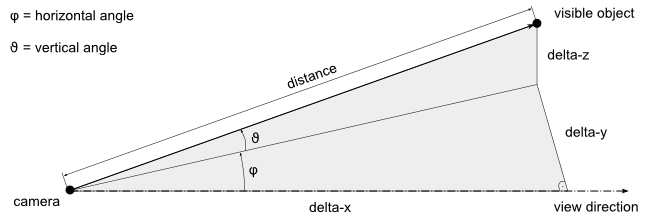
\includegraphics[width=10cm]{images/Vision_Perception.png}
\caption{RoboCup agent visual perception \citep{perceptors}}
\label{fig:spherical}
\end{center}
\end{figure}

Low level control of the agent is abstracted by using magmaFatProxy-1.2.2, which also needs to be extended to include the handling of image messages.

\subsection{Preprocessing}

The images are decoded into an RGB array format that can be displayed, manipulated and stored using the Numpy and OpenCv Python libraries. In order to better understand the performance of each detector in the context of the image content, images are sorted into categories that classify ball visibility, occlusion, size as well as play mode. Hidden and occluded ball images must be manually separated, since the server vision messages do not include the breakage of line-of-sight (all objects are transparent to the agent).

From the spherical coordinates of the ball that are given by the match server relative to the center of the head of the Nao agent, one can transform them to the camera position by converting the coordinates to a Cartesian axis, performing a translation (given 6.5cm head radius) and then returning the coordinate system to spherical. From the spherical coordinates at the camera, with the known 58\textdegree\ field of view of the camera, it is possible to use an ideal wide angle lens transformation to determine the BB center in image coordinates. This transformation is based on the ideal fish-eye lens model (See figure \ref{fig:wideangle}) which is then extended to the two rotational axes using spherical geometry. The size of the bounding box is then determined based on the distance of the ball (with known 8.4cm diameter) and the expected size on the optical projection plane.

\begin{figure}[h!]
\begin{center}
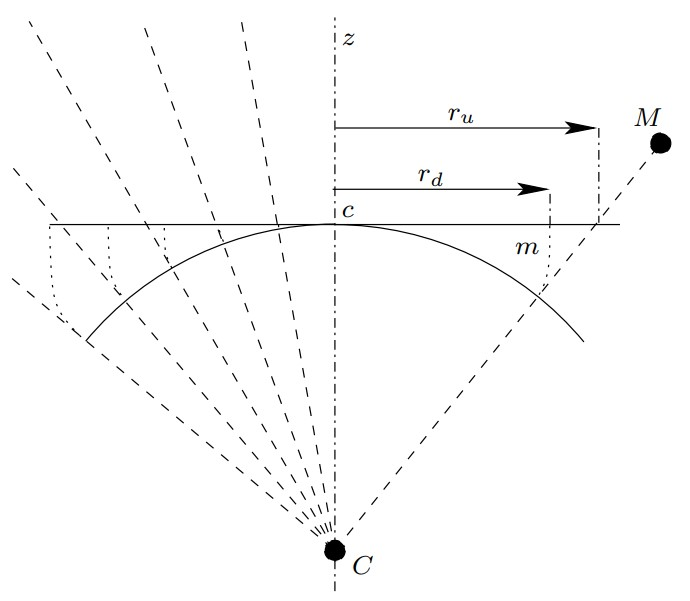
\includegraphics[width=6.5cm]{images/FOVmodel.jpg}
\caption{Ideal wide angle lens transformation \citep{wideangle} }
\label{fig:wideangle}
\end{center}
\end{figure}

Although the transformations can automatically be computed to get BBs for all ball containing images, using the simulator to produce perspective images for control purposes is outside of the typical usage of the simulator - it is found that in some agent initializations (approximately 1 in 5) that the synchronization of the produced images to the ground truth is between time steps and the temporal misalignment visually obvious. In these cases the data is dropped, however, it requires a manual process of inspecting ground truth bounding boxes as a way of detecting bad initializations was not found.

Each object detector expects the dataset to be presented in a certain structure with annotations in a specified format in order to facilitate dataloading. NanoDet utilizes the COCO format \citep{cocodataset} which is commonly used by recent detectors, whereas the VJ detector expects a bespoke format \citep{vjdataset} and YOLO uses a ``Darknet'' format. Scripts are made to automate these conversions respectively from the .json formatted data. A 60:20:20 training, validation, test split is used.

\subsection{Data Exploration}
The dataset is interrogated in order to understand and sanity check the acquired data and the randomly sorted splits. Table \ref{tab:detection} shows a break down of various image properties. The size of the object is classified according to \cite{cocoeval}, which declares small objects as those less than $32\times32$ pixels and large as greater than $64\times64$ pixels. Occluded images are any where a percentage of the pixels of the ball are hidden.

\begin{table*}[h!]
\fontsize{9.5pt}{12pt}\selectfont
\centering
\begin{tabular}{c|ll|lll|ll|lll}
{\bf Dataset}	&{\bf Count}	&{\bf Split}	&{\bf Visible}	&{\bf Hidden}	&{\bf Occlu.}	&{\bf Match}	&{\bf Drill}	&{\bf Small}	&{\bf Med.}	&{\bf Large}	\\\hline
Total			&2563			&100\%			&70.6\%			&20.1\%			&9.3\%			&50.6\%			&49.4\%			&54.6\%			&25.1\%			&0.2\%			\\\hline   
Train			&1537			&60\%			&70.4\%			&20.3\%			&9.3\%			&51.0\%			&49.0\%			&53.5\%			&26.2\%			&0.1\%			\\\hline  
Validation		&513			&20\%			&72.9\%			&18.9\%			&8.2\%			&51.1\%			&48.9\%			&58.3\%			&22.8\%			&0.0\%			\\\hline  
Test			&513			&20\%			&68.8\%			&20.9\%			&10.3\%			&70.6\%			&50.9\%			&54.2\%			&24.4\%			&0.6\%			\\\hline                        
\end{tabular}
\caption{Detection dataset}
\label{tab:detection}
\end{table*}

With the data acquired using the target environment, it is expected that the dataset is representative. It is seen that the properties are consistent through each split. The majority of the images have a visible ball (since the agent looks for the ball). There are a non-negligible number of occluded ball images since a match environment features many obstructing players. Further, its clear that small bounding boxes are the majority of the cases, with large being very infrequent. This is to be expected.

The ground truth BBs are plotted with some examples of the dataset in figure \ref{fig:detectimages}:

\begin{figure}[h!]
\begin{center}
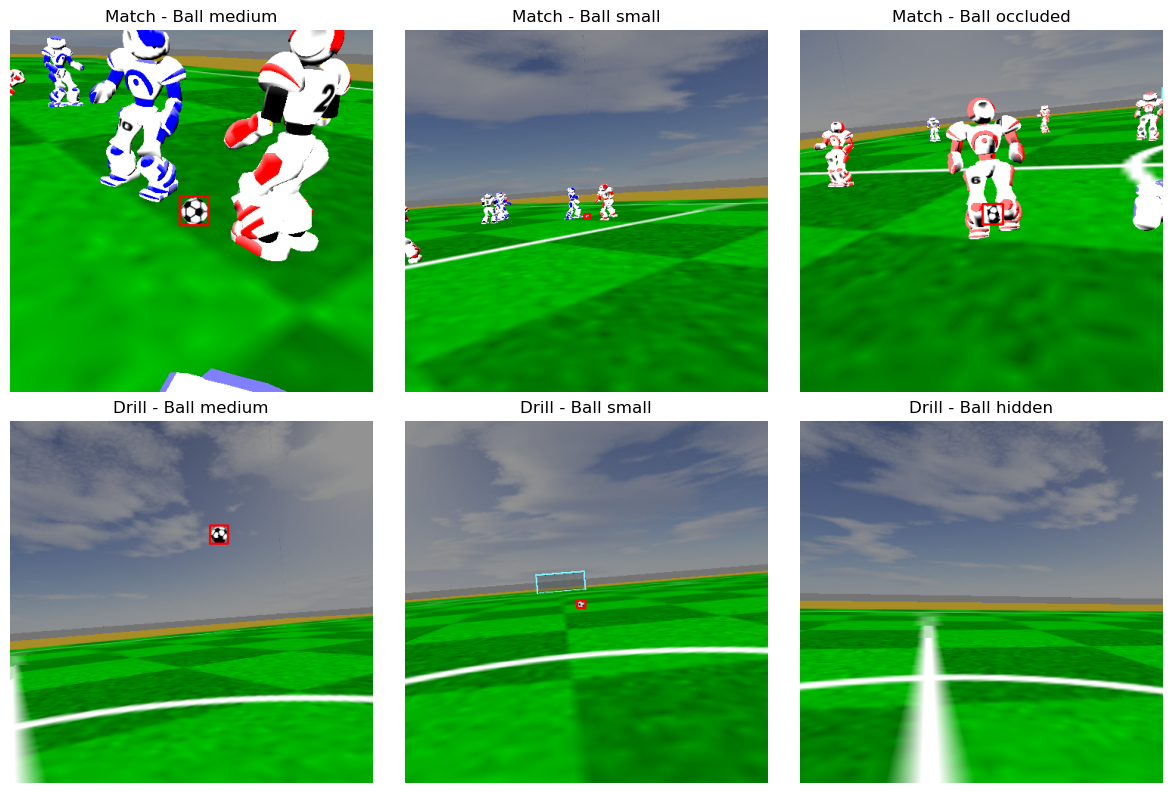
\includegraphics[width=16cm]{images/imagedetections.png}
\caption{Detection dataset ground-truths}
\label{fig:detectimages}
\end{center}
\end{figure}

The bounding box characteristics are plotted in figure \ref{fig:detectplot}. It is seen that the ball has a bias to be found in the center of the agent perspective, this is caused by the agent which tends to focus on the ball. Data augmentation such as cropping can be used to avoid over-fitting on this trait.

\begin{figure}[h!]
\begin{center}
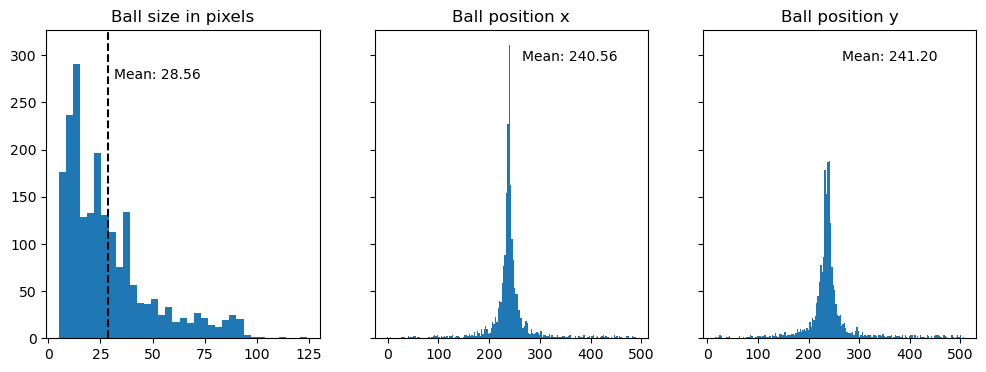
\includegraphics[width=15cm]{images/plotdetections.png}
\caption{Detection dataset ball statistics}
\label{fig:detectplot}
\end{center}
\end{figure}

\section{Baseline detection}

The baseline detectors, which have been chosen based on known prior usage in RoboCup as seen in the related works, are now investigated.

\subsection{Viola Jones}

The Viola Jones classifier (more generally known as the haar cascade classifier) is implemented in the OpenCV libraries. It can be trained, stored and loaded for performing inference. A multi-scale implementation is utilized which, applies a scaling factor ($scaleFactor$) that reduces the image size to create an ``image pyramid'' to evaluate different object sizes with the same detector. 

In the following section, the steps taken to prepare the software environment and data are described. Following this the training process, which aims to maximize the quality of the inference is discussed. Finally, an ablation study is performed to maximize real-time performance of the detector.

\subsubsection{Software environment}

It is found that OpenCV no longer supports the training of Viola Jones style detectors from version 4 onwards due to dropping support of the legacy C API (although, inference is still supported). Therefore it is chosen to roll back and build the OpenCV 3.4 release. The official documentation by \cite{vjdataset} is used.

\subsubsection{Data preparation}

In the spirit of the related works of \cite{robovj}, for ball detection, a pipeline is created where the camera image is edge filtered and a hand crafted threshold applied to create a crisp binary image as an input feature. 

With the detection data prepared and structured accordingly, the $opencv\_createsamples$ application is used to create positive examples by cropping the objects using the ground truth bounding boxes and storing them in a binary format (vec-file). The size ($w\times h$) of the positive examples must be specified and must match the window size of the classifier to be trained. The \cite{vjdataset} recommendation is to use the size of the average object as the window dimensions - which in this case is $28\times 28$. The output is shown in figure \ref{fig:edgeball} (gray pixels caused by interpolation during rescaling).

\begin{figure}[h!]
\begin{center}

\includegraphics[width=2cm]{images/edge32.png}
\caption{Thresholded edge image}
\label{fig:edgeball}
\end{center}
\end{figure}

\subsubsection{Model training}

The training of the detector is done as described by \cite{vjdet}. In this approach, rather than trying to perform an optimization of the number of stages, features per stage and threshold per stage -- which is considered to be a difficult problem -- a goal is chosen for the desired minimum hit rate and the desired maximum false alarm rate for each stage of the classifier. Each additional layer reduces the false alarm rate but also the hit rate, layers of features are added until the goal is met.

The hit rate defines the amount of positive object training data that must be correctly classified. A higher hit rate prevents overly confident features that can cause positives to be incorrectly classified. The overall hit rate is computed as:
\begin{equation}
Overall\_hitRate = hitRate^{numStages}
\end{equation}
False alarm rate sets the rate at which false positives may occur. A lower number requires more weak classifiers to reject negatives correctly which therefore dictates how many features (also known as layers) are included in each stage. 
\begin{equation}
Overall\_falseAlarmRate = falseAlarmRate^{Num\_Stages}
\end{equation}
The number of features used is then increased until the target rates are met for this stage. Training further stages is usually stopped early if $acceptanceRatio$ (negative samples wrongly classified as positive) is reached, which prevents over-fitting of training data. In this study, a search is performed over $numStages$, and evaluated for the AP score against tested and validation sets, in order to ensure that the model is both sufficiently trained but also not over-fitting, for the actual targeted detection task.  

In line with \cite{robovj} $minHitRate = 0.999$ is chosen. A search for $falseAlarmRate$ is performed, which when coupled with $numStages$ allows for a variety of $Overall\_hitRate$ and $Overall\_falseAlarmRate$ combinations to be evaluated. $numPos$ is chosen to be 90\% the positive samples, providing a conservative buffer of images to compensate for the cases falsely not detected by the classifier. A common choice for $numNeg$ is twice $numPos$. The remaining parameters are recommended values by \cite{vjdataset}.

\begin{figure}[h!]
\begin{center}
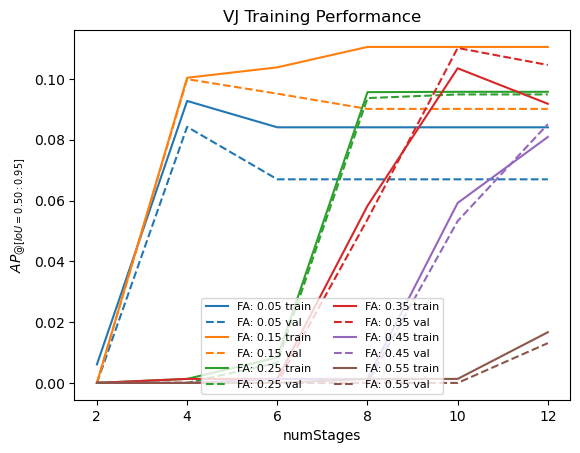
\includegraphics[width=10cm]{images/vj_training.png}
\caption{AP vs $numStages$}
\label{fig:vjstages}
\end{center}
\end{figure}

With some difficulties obtaining GPU support, CPU based training was performed using a computing cluster hosting Intel Xeon E5-2680 processors. The speed up achieved using OpenMP was sufficient to allow reasonable training times. Adding additional stages coincided with an increased training time, with the longest for 12 stages being roughly 6 hours. Initially, it can be seen on the training curves (figure \ref{fig:vjstages}) that the addition of stages allows the model to better fit the data, which leads to convergence - a show of sufficient training. However, the further addition of stages can lead to over-fitting which results in a decrease in validation performance. In general, the validation and training scores are not significantly different, which indicates that sufficient training examples are provided and that the datasets are reflective. The best performer on the validation set ($FA=0.35$) is chosen for further optimization.

The first layers of the final stage can be visualized in figure \ref{fig:vjlayers}:

\begin{figure}[h!]
\begin{center}
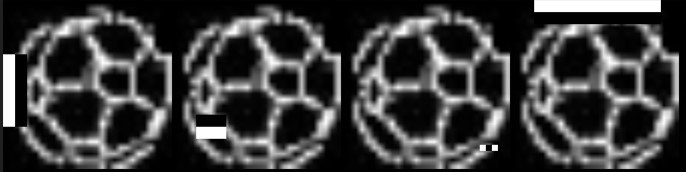
\includegraphics[width=9cm]{images/vj_result.jpg}
\caption{Cascade classifier 4 layers of final stage}
\label{fig:vjlayers}
\end{center}
\end{figure}

In the layers investigated, it can be observed that the model seems to learn: the outer boundary of the ball, the thickness of the edges as well as the patches of the ball. These make intuitive sense and provide confidence in the results that have been obtained.

During inference, $minNeighbors$ provides a measure of confidence to retain the candidate, which is fine-tuned on the validation set to maximize the AP score (figure \ref{fig:vjneighbors}).

\begin{figure}[h!]
\begin{center}
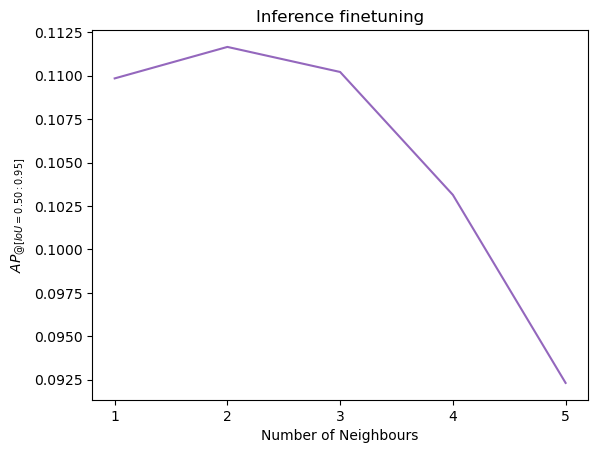
\includegraphics[width=9cm]{images/vj_tune.png}
\caption{AP vs $minNeigbours$}
\label{fig:vjneighbors}
\end{center}
\end{figure}

\subsubsection{Model tuning}

An ablation study is now performed in order to optimize accuracy in the context of a real-time performance. A search is performed to optimize the $scaleFactor$ (figure \ref{fig:vjspeeds}).

\begin{figure}[h!]
\begin{center}
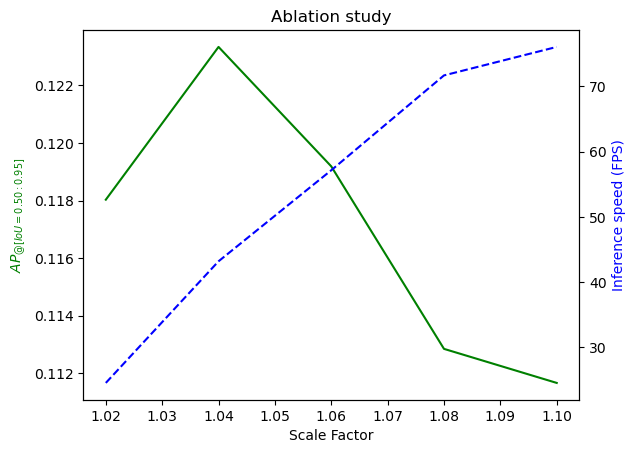
\includegraphics[width=11cm]{images/vj_ablation.png}
\caption{AP, latency vs $scaleFactor$}
\label{fig:vjspeeds}
\end{center}
\end{figure}

\subsection{YOLO v4 Tiny}

YOLO object detection is based on the Darknet deep learning framework, which is purpose built for training and evaluating the YOLO architecture in the object detection task. Alongside the framework, the pretrained YOLO v4 Tiny \citep{yolov4tiny} model from the author is made available, which has been pretrained on the COCO dataset, as well as the configuration and pretrained backbone that have been used to get the reported results. Since the COCO dataset features a ``sports ball'' category, it is possible to apply the pretrained model to the Robocup ball dataset in order to evaluate how well the models generalize between the domains as well as getting a feel for the performance gain that can be achieved at the cost of additional training.

In the following section the steps taken to prepare the software environment and data are described in order to train YOLO v4 Tiny on the RoboCup dataset. Trained models of this framework are represented and stored by a configuration file and weights file. External tooling can be used to convert the results into the desired ONNX format. 

\subsubsection{Software environment}

 The ``YOLO V4'' release is cloned from the official repository hosted on github \citep{yolov4repo}. Before compiling the framework on the target training hardware, CUDA 11.8 is linked in the makefile - in order to benefit from GPU acceleration. The training dataset needs to be prepared in a ``Darknet style'' format, therefore a script is created to do this. The web service ``Roboflow'' \citep{roboflow} is utilized as a means of validating the produced annotations by importing and visualizing the data. 

\subsubsection{Model training}

The release configuration for YOLO v4 Tiny was utilized for model training which uses the CSPDarknet53 backbone (pretrained on ImageNet). Links to these can be found hosted on the Github repository \citep{yolov4repo}. As part of the ``bag-of-freebies'' training approach which can boost accuracy without an increase of the inference cost, a set of augmentations -- such as photometric and geometric distortions as well as simulated object occlusion are applied. To train the network, a multipart loss is minimized. The classic YOLO objective function has the following high level form:
\begin{equation}
L_{YOLO} =  L_{cls} + \lambda L_{reg} + \lambda' L_{confi} 
\end{equation} 
Where $\lambda$ and $\lambda'$ are balancing parameters used to weigh each term -- giving importance to bounding box regression and decreasing the importance of boxes not containing objects (AKA ``noobj'') respectively. $L_{cls} $ refers to the class prediction which is represented by the focal loss. $L_{confi}$ refers to the objectness score (which is the probability that and object is present) which is represented by the $L2$ loss. $L_{reg} $ refers to the bounding box regression loss. YOLOv4 applies a loss known as ``Complete-IOU'' (CIoU) \citep{diouloss} (rather than $L2$ loss) which offers an objective which is made to suit to the IoU evaluation metric. CIoU is an incremental improvement over ``Generalized-IoU'' (GIoU) \citep{giouloss} which solves the ``gradient-vanishing`` problem resulting from a basic IoU loss which would only ``work'' when the bounding boxes have overlap. 

Initial trials showed that compiling the framework without any of the performance enhancing dependencies led to model training being estimated at over 200 hours to achieve completion, which was unacceptable. This was reduced by an order of magnitude if OpenMP was included for parallelizing and then by a further order of magnitude if CUDA was included for GPU acceleration of the training passes. A cluster hosting NVIDIA GeForce GTX 1060 processors was utilized, resulting in a model training time of approximately 2 hours which is a significantly more manageable duration. The recommended number of cycles by the author is applied for training, which is 2000 epochs per class but no less than 6000 overall.

The models are trained across various resolutions in order to investigate the speed/accuracy trade off and make a sensible selection of a real-time solution. It should be noted that model image resolutions need to be in multiples of 32 due to the model architecture.

\begin{figure}[h!]
\begin{center}
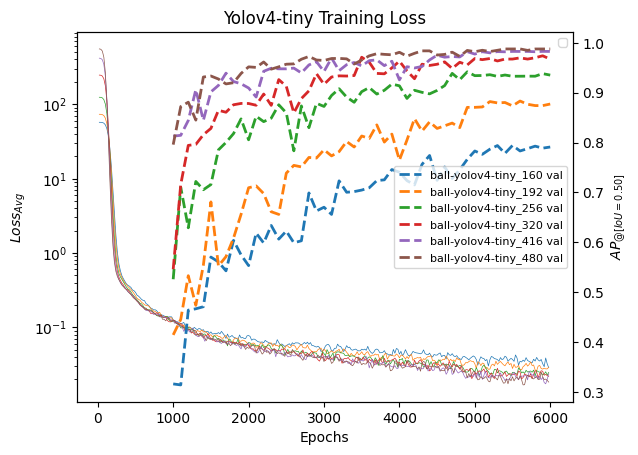
\includegraphics[width=13cm]{images/yolov4tiny_train.png}
\caption{YOLO v4 Tiny training curves}
\label{fig:yolov4tiny_train}
\end{center}
\end{figure}

In figure \ref{fig:yolov4tiny_train} it is seen that for each model, as the number of training epochs is increased the loss score decreases. This corresponds to the model learning the structure of the training dataset and performing better inference on each training example. Initially a very high rate of learning is achieved which reduces over time, however, it does not yet plateau. Too much training can lead to the model over-fitting the training dataset which can harm the ability of the model to generalize to the task it is training for. The model is also evaluated against the validation dataset every 10 epochs, which provides a measure of how well the model captures the general relationships in the data. After 5000 Epochs, it is clear that a plateau in the validation performance has occurred which is a good indicator that sufficient training has been performed. 

\begin{figure}[h!]
\begin{center}
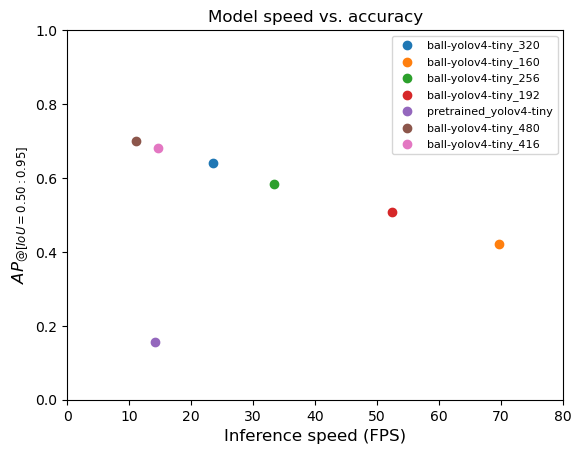
\includegraphics[width=10cm]{images/yolov4tiny_compare.png}
\caption{YOLO v4 Tiny variations compared}
\label{fig:yolov4tiny_compare}
\end{center}
\end{figure}

It can be noted that the $AP_{@[IoU=0.5]}$ score of the $480 \times 480$ resolution model achieves a near perfect result. This gives confidence that although the architecture has been prepared for the COCO dataset, it is capable of capturing the patterns within the data without the cost of a comprehensive search for hyperparameters. As the model resolution is decreased, the quality of the inference decreases. The models are also evaluated for inference speed, shown in figure \ref{fig:yolov4tiny_compare}. A reduced resolution allows faster inference. In order to achieve real-time inference, a significant drop in resolution from $480 \times 480$ down to $256 \times 256$ is required. This results in a drop in achievable inference quality.

The additional data point of the pretrained model is also included. Although this model evaluates 80 COCO classes at $416 \times 416$, there is no significant difference in inference speed when compared to the trained model which only searches for the ball class. In principle this means that the detector can be extended to include limited additional classes such as the goal posts and other agents without significant time consequence.

\section{Proposed detection}

Initially, a simple naive study is performed to justify the selection of the NanoDet object detector. Then, the detector is trained in order to find the most suitable configuration.

\subsection{Naive latency evaluation}
In order to justify the selection of a modern real-time object detection architecture, a naive approach is taken to simply evaluate pretrained models on the target device. In this approach, only the latency of the forward pass is considered and the accuracy of the detentions is ignored. In this manner, a coarse approximation of the performance can be acquired. Further, the size of the model is also considered as a secondary factor.

The models are gathered in the following manner. All detector models from the ONNX model zoo \cite{modelzoo} are used. NanoDet was found to be the most promising model, therefore more pretrained NanoDet models of different configurations were gathered and converted to ONNX format from the official repository for exploratory purposes. YOLOX \citep{yolox} is also a recent anchor free approach which may be a suitable alternative to NanoDet - therefore a pretrained detector is taken from its official repository \citep{yoloxrepo} and also converted to the ONNX format. YOLOv5 is readily accessible in the pytorch library and is included due to its ease of access. 

In this experiment, a 15 second perspective sequence (375 frames at 25hz) of RoboCup gameplay is preloaded as an array of $m \times n \times c \times frames$. The average time to complete inference of all frames is recorded and plotted alongside model size in figure \ref{fig:modelspeedsize}. The detectors have been evaluated using onnxruntime 1.12.1 on a single core of an AMD Ryzen 5 4600H CPU, limited to single threaded execution using the session option $intra\_op\_num\_threads = 1$. The faster models tend to have less mathematical operations, and therefore also have less weights which results in smaller model sizes. Compared to the 1GB of RAM available on the Nao v5, the models larger than 50mb are certainly difficult to accommodate and larger than ONNXruntime linux binary itself ($\approx13mb$).

\begin{figure}[h!]
\begin{center}
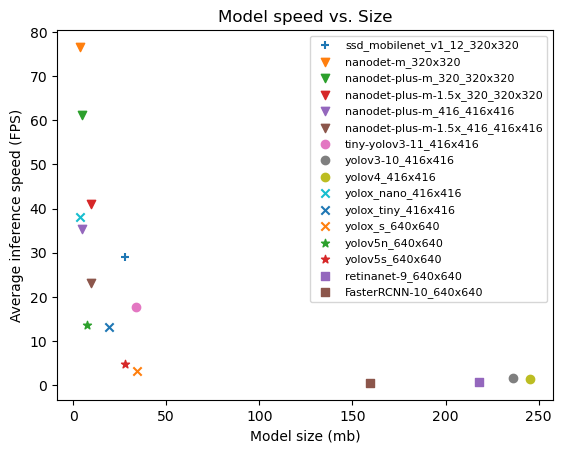
\includegraphics[width=10cm]{images/modelspeedsize.png}
\caption{Pretrained model performance vs. size}
\label{fig:modelspeedsize}
\end{center}
\end{figure}

\begin{figure}[h!]
\begin{center}
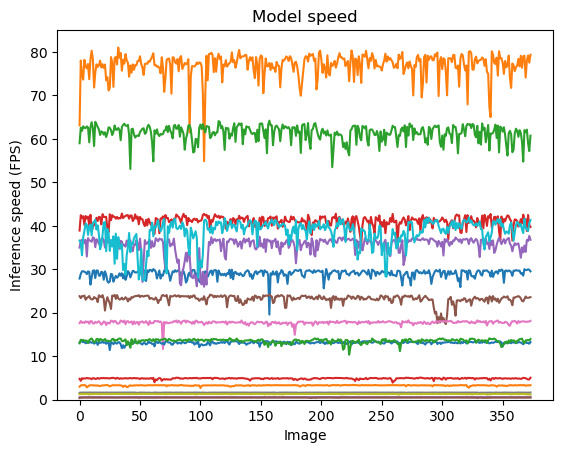
\includegraphics[width=10cm]{images/modelspeed.png}
\caption{Pretrained model performance}
\label{fig:modelspeed}
\end{center}
\end{figure}

It is found that most of the detectors do not execute in real-time on this hardware. Although, this does not definitively mean that they cannot (after model tuning) but rather demonstrates that one will likely sacrifice a significant amount of inference quality to achieve this. Therefore these are not ideal choices to pursue. It is found that NanoDet executes in real-time for many of its configurations and therefore is a good choice to investigate further. The inference speed does fluctuate due to other processes which share the same computational resources. Therefore, for the best real-time results, one should aim to compute slightly faster than real-time to avoid latency issues. 

\subsection{NanoDet}

The NanoDet object detector is built using PyTorch which is a popular general purpose deep learning framework. Models can be trained, stored and loaded for performing inference in Python. The NanoDet repository can be found on github with tested pretrained models for the COCO dataset which are shared by the authors \citep{nanodet}. Some variations of the model exist such as the ``Plus'' architecture which is the most recent and best performing architecture. A formal paper is not available.

%In the following section, the steps taken to prepare the software environment and data are described. The training and model selection process is reported which has been used to deliver a suitable detector.

\subsubsection{Software environment}

NanoDet-Plus v1.0.0 (d3fb34f) is cloned from \cite{nanodet}, which is the latest release of the repository at this time. The PyTorch deep-learning framework is used however only versions $<$ 2.0.0 are supported which must be therefore be manually installed, rather than using the currently outdated instructions found on the repository, before installing the required packages to get a suitable environment. It should also be noted (since it is not documented) that the ``Plus'' architecture has a different output shape, which may cause frustration for researchers that are using previous work.

\subsubsection{Model training}

During an initial study using the pretrained model, it is found that the model achieves a useful performance on the target dataset (see figure \ref{fig:evaldetect}) - even though it is synthetic. This supported the approach of fine-tuning the pretrained model onto the RoboCup ball dataset. The NanoDet model expects the data to be structured and annotated in a COCO style format, therefore a script is created to do this. The web service ``Roboflow'' \citep{roboflow} is utilized as a means of validating the produced annotations by importing and visualizing the data. 

In order to train the network, a multipart loss must be minimized. The NanoDet objective function can be understood by the following high level form:
\begin{equation}
L_{NanoDet} =  L_{GFL}(L_{QFL}, \lambda L_{DFL}, \lambda' L_{GIoU})
\end{equation} 
Generalized Focal Loss (GFL) \citep{gflloss} generalizes Focal Loss from a discrete form to a continuous form -- which results in improvements to network training. GFL unifies Quality Focal Loss (QFL) and Distributed Focal Loss (DFL) where QFL is a joint representation of localization quality and classification -- which softens a typical one-hot category label to a float representation of each category -- and DFL softens the representation of bounding box regression by viewing the offsets from the predicted center to the bounding box boundaries as a continuous arbitrary distribution rather than deterministically.

A variety of the release NanoDet architectures - which have been shared by the authors - are chosen and the default parameters and augmentations are utilized. Again, NVIDIA GeForce GTX 1060 processors are available for training. The training curves shown in figure \ref{fig:nanodet_train} compare the training and validation results.

\begin{figure}[h!]
\begin{center}
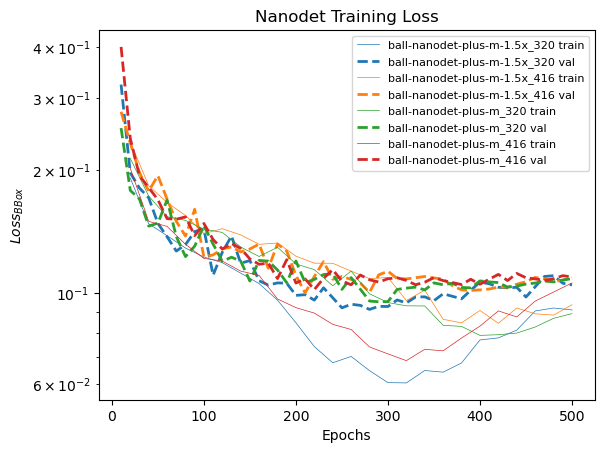
\includegraphics[width=13cm]{images/nanodet_train.png}
\caption{NanoDet training curves}
\label{fig:nanodet_train}
\end{center}
\end{figure}

In general, it can be seen that as more epochs are performed, the loss scores are reduced. This indicates that the model is learning the training data and improving its ability to perform object detection. Further, it can be seen that as training epochs are performed the validation scores of each of the models increases. This indicates that the model is indeed learning the general structure of the data. After a number of epochs have been performed, the validation scores reaches a pleateu. This indicates that sufficient training iterations have been performed and that further training may lead to over-fitting of the training data. The best iteration of each model is chosen based on the validation AP scores. 

Post training, repository provided tools are used to produce the model in an ONNX format. A crucial step not documented by \cite{nanodet} is to post-process the ONNX model with the ONNX runtime $remove\_initializer\_from\_input$ function. Without this, a significant degradation in inference speed occurs, preventing the detector to run in real-time. The different NanoDet variations are evaluated for their inference speeds and their performances are plotted in figure \ref{fig:nanodet_compare}.

\begin{figure}[h!]
\begin{center}
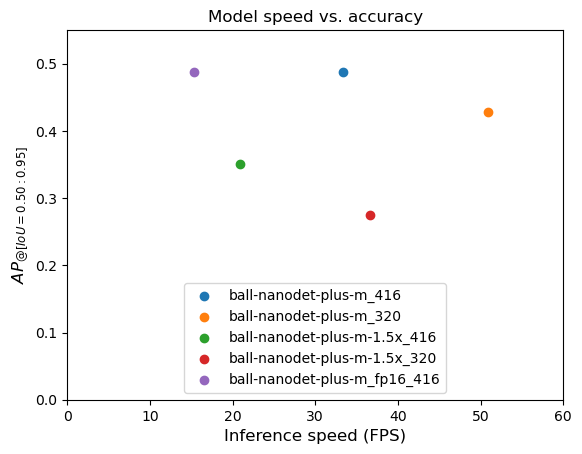
\includegraphics[width=10cm]{images/nanodet_compare.png}
\caption{NanoDet variations compared}
\label{fig:nanodet_compare}
\end{center}
\end{figure}

The validation scores for NanoDet are the highest of any of the considered models, without even performing a search for hyper parameters. For this reason, the additional efforts of a search is not performed (beyond the included basic architecture variations) as the results are satisfactory and sufficient to prove the respective hypothesis. 

Similar to the results of all models considered thus far - it is seen in general, that the higher resolution architectures ($416 \times 416$ vs. $320 \times 320$) perform inference at a higher accuracy, however, at a cost of inference speed. The $1.5\times$ models -- which have a deeper backbone -- also perform inference slower, however, in this case they do not perform at a higher inference quality. A reason for this could be that more complex models are prone to overfitting the pretraining data as they are able to capture the complex characteristics that are only present in the training data. The ``NanoDet-plus-m\_416'' instance is chosen as it provides the maximum performance at a speed that provides real-time inference.

%Additionally due to an increased network complexity they may also be more sensitive to hyperparameters - since models of greater complexity have a greater tendancy to overfit and the chosen parameters here are optimised for the COCO different dataset.

In order to investigate model optimization for deployment, the chosen model is quantized from a float32 to a float16 representation - which gives a resulting model size reduction from 5.5mb to 3.2mb. A negligible loss of inference quality is realized but a significant reduction in speed has occurred. The reason for this appears to be that that float16 operations is not well supported by all hardware (x86 CPUs) and thus require conversion to a float32 representation which adds an overhead. Since the model is already of acceptable size compared to the size of the ONNX Runtime binary, the quantized model is not utilized and further quantization is not investigated.

\section{Evaluation of detection}

The selected pretrained, trained and fine-tuned networks of the various object detection models are now compared relative to each other using the test dataset which has been isolated and remained unseen thus far. The dataset is decomposed into object sizes, scenario and occlusion for evaluation which helps to provide an insight into the performance of the detectors across various circumstances. 

The object detection data is evaluated in three stages. Firstly, the ``easiest'' data is used, which does not feature match environment images or occluded images. This is most representative of the tracking portion of the research. Then, the dataset is extended to included match images (but not occluded images). It is thought that such a set would expose the model performance among a more challenging and dynamic background which is reflective of a RoboCup soccer environment and more likely to result in false positives. Finally, occluded images are added in, which helps to provide an indication of the performance against complex images with only partial object information. This provides the most realistic performance evaluation in a typical simulated soccer scenario. 

The results are plotted in figure \ref{fig:evaldetect}. Various conclusions can be drawn from these results, which are discussed below:

\begin{figure}[h!]
\begin{center}
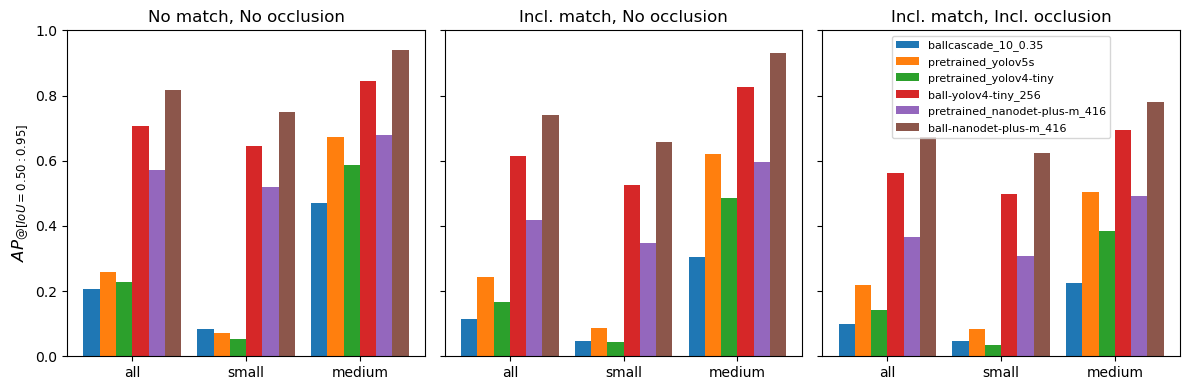
\includegraphics[width=15.5cm]{images/eval_detect.png}
\caption{Evaluation of detectors}
\label{fig:evaldetect}
\end{center}
\end{figure}

\subsubsection{Performance against increasing difficulty}

As a whole - it is observed that the models perform worse on the datasets of increased complexity, which is expected. Match images cause a decline in performance as the ball is more difficult to identify among the agents. The distance of the ball also corresponds to decreased performance as smaller objects are more difficult to classify and regress accurately. Additionally, occluded images cause even further performance decline as it provides only partial information for inference. A contributing factor towards this is that challenge of accurately predicting the bounding box. In particular, object detection models tend to place boundaries bound around the visible part of the object, whereas for tracking the bounding box should also border the parts of the ball that are unseen in order to estimate distance. 

\subsubsection{Traditional detection}

Relatively, the VJ detector performs the worst of any of the detectors across the data. Despite the effort of searching for ideal parameters, performing tuning and the trouble of training, it does not out perform any trained detector. Infact, the pretrained detectors provide better inference quality without any training effort and framework complexity. With the ease of the modern frameworks and performance of the models versus the minimal support and bespoke OpenCV tooling needed for training the VJ detector, it is obvious why utilizing the older models for new applications has fallen out of favor. When a ball is correctly identified (as in figure \ref{fig:evalvjnano}), a further challenge appears to be the tightness of the fit of the bounding box due to the sliding window approach.

\begin{figure}[h!]
    \centering
    \subfloat{{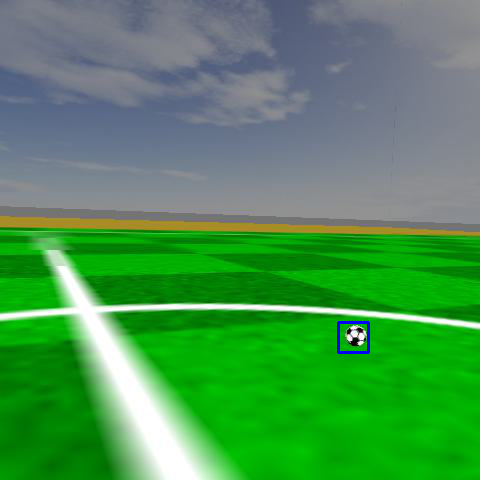
\includegraphics[height=5cm]{images/eval_vj.png}}\label{fig:evalvjnano}}
    \qquad
    \subfloat{{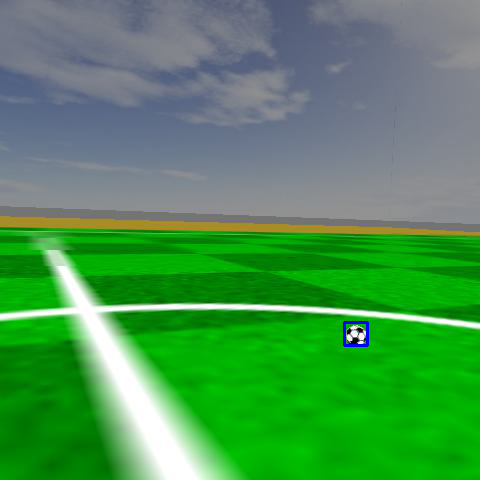
\includegraphics[height=5cm]{images/eval_nanodet0.png}}}
    \caption{Trained Viola Jones (Left) and Trained NanoDet (Right)}
\end{figure}
\vspace*{-0.5cm}
\begin{figure}[h!]
    \centering
    \subfloat{{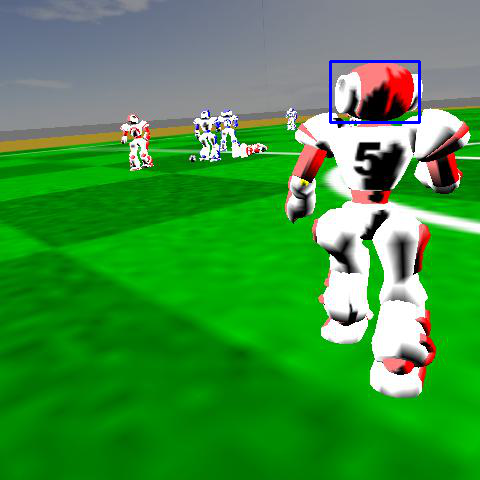
\includegraphics[height=5cm]{images/eval_nanodetpre.png}}\label{fig:evalnanonano}}
    \qquad
    \subfloat{{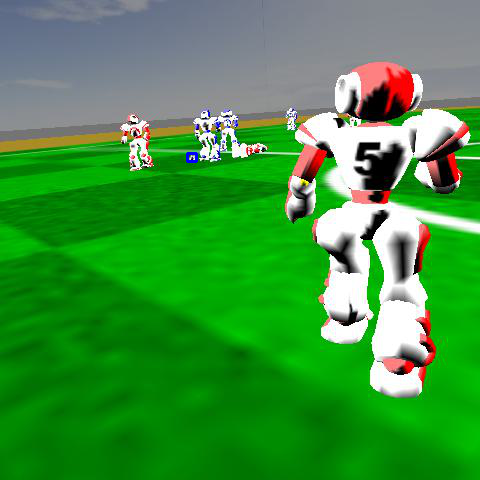
\includegraphics[height=5cm]{images/eval_nanodet1.png}}}
    \caption{Pretrained NanoDet (Left) and Trained NanoDet (Right)}
\end{figure}

\subsubsection{Pretrained modern detection}

One of the interesting results that can be seen is that the pretrained detectors chosen actually achieve a useful performance on the unseen and synthetic RoboCup ball tracking dataset - although only for medium size objects (likely due to the COCO dataset under-representing small objects \citep{smallcoco}). This is not a generalization that one can necessarily rely on for all synthetic datasets, however, it is a useful result for expressing the domain adaptive property of the models and may be helpful for informing an initial selection of suitable algorithms that are susceptible to a task.

\subsubsection{YOLO v4 Tiny}

The YOLO v4 Tiny model shows significant improvements in performance and surpasses the VJ detector in all categories in terms of inference quality. Initially the pretrained model suffered from poor inference of small objects but after training a significant boost in performance was realized. However, in order to achieve a real-time performance the quality of inference had to be significantly reduced. This result corresponds to the results seen in the related works, where it was found that the YOLO v4 Tiny model does perform well in the task of RoboCup ball detection, however, these results do not carry over to real-time speeds. An unfortunate result is that the performance of the model against distance balls significantly drops in a match scenario. This reflects that the model has a tendency toward false positives, confusing the ball with the agents. This is seen in figure \ref{fig:evalyolonano} where the boundary of the prediction slightly extends to include the agent behind the ball. Storage of the model weights is approximately 30mb which is larger than the binary of ONNX Runtime but still manageable with the given memory of a typical Nao RoboCup platform.

\begin{figure}[h!]
    \centering
    \subfloat{{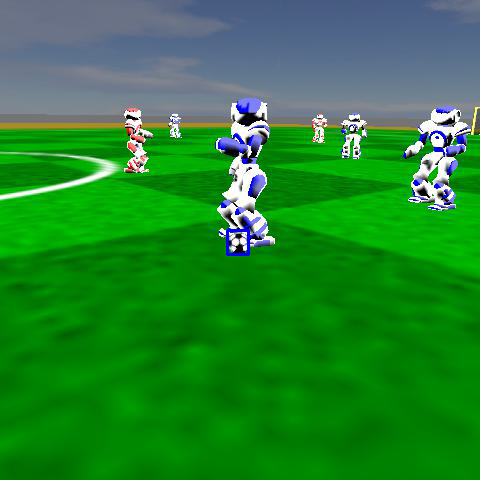
\includegraphics[height=6cm]{images/eval_yolo.png}}\label{fig:evalyolonano}}
    \qquad
    \subfloat{{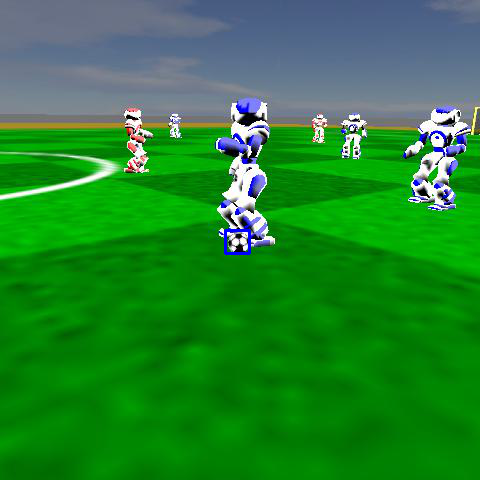
\includegraphics[height=6cm]{images/eval_nanodet2.png}}}
    \caption{Trained YOLOv4 (Left) and Trained NanoDet (Right)}
\end{figure}

\subsubsection{NanoDet}

The NanoDet model shows itself to be the best network across all scenarios by out performing all other architectures at real-time speeds. This is true across each dataset characteristic and by a significant margin. A key insight that can be observed is that the pretrained Nanodet is the only pretrained model which has a useful performance for identifying at the small size balls (long range). This is interesting since the pretrained YOLO v4 Tiny model has also been trained for optimum performance against COCO but has no comprehension before training. Further, for the easiest scenario, the trained NanoDet scores a near perfect result which is impressive. This model also has the smallest memory footprint, only utilizing 5mb of storage capacity. For limited capacity machines this allows the memory to be used for other tasks, helping to improve the overall performance of the robotic platform. Therefore, for a ball detection system that may be used in a match scenario or for the proposed tracking, NanoDet is chosen.

%%%%%%%%%%%%%%%%%%%%%%%%%%%%%%%%%%%%%%%%%%%%%%%%%%%%%%%%%%%%%%%%%%%%%%%%%%%%%%%%%%%%%%%%%%%%%%%%
\chapter{Object tracking investigation}

\section{Tracking dataset}
As before, the dataset is generated using various open source programs in the RoboCup soccer ecosystem as well as the Wits agent with a bespoke behavior. Each kick is randomized and then captured in a practice environment as a sequence of images (with metadata) at 25hz with respective ground-truth positions at 50Hz.

\subsection{Software environment}
The kick tracking data is also generated using the RoboCup match server rcssserver3d-0.7.3 and simspark-0.3.2 simulator using the same settings as used for the detection dataset. Additionally, in the match server: a ball and agent ground truth perceptor is added to append global ball and agent positions to the server messages. The limit of the agent ``BeamEffector'' is changed to extend the beam-able area of the agent into the opposition half in order to ensure that the dataset has full coverage of the arena.

Alongside producing .json files for image with metadata as before, the Wits agent stores a .csv file for each kick sequence which captures, for each time step, ground-truth positions as well as the agent transformation matrices from the Nao head coordinate system though the agent torso to the global coordinate system. The camera transformation used is the inverse from the detection dataset - taking a bounding box at the camera position to a spherical coordinate located at the center of the agent head. The data is synchronized by the server time. Low level control of the agent is also abstracted by using magmaFatProxy-1.2.2, but the code needs to be extended to enable the server to handle ground truth ball and agent position messages without crashing. 

\subsection{Preprocessing}

A small portion of the tracking sequences need to be discarded due to abnormalities such as: agent instability, kicking outside of the play area and ball rebounding off the goal posts. These edge cases occur infrequently enough to ignore for training, however, are manually excluded by watching the sequence. 

In order to conserve memory, the tracking sequence images are taken from their .json base64 encoded string and compressed into an .avi video format - which results in a 99\% reduction in size from 100mb per sequence. However, a dataloader is required to be constructed which also ensures synchronization between image and metadata.

\subsection{Data exploration}

The dataset is interrogated in order to understand and sanity check the acquired data. Table \ref{tab:tracking} shows a break down of various sequence properties. Kicks that have a peak height above the height of the diameter of the ball are deemed to be lofted. As seen in figure \ref{fig:plotkicks}, lofted kicks have a trajectory that is dominated by bouncing behavior compared to ground kicks which roll.

\begin{table*}[h!]
\fontsize{9.5pt}{12pt}\selectfont
\centering
\begin{tabular}{c|ll|l|ll}
{\bf Dataset}	&{\bf Kicks}	&{\bf Split}	&{\bf Mean steps}	&{\bf Grounded}	&{\bf Lofted}	\\\hline
Total			&370			&100\%			&295.4			&20.3\%			&79.7\%			\\\hline   
Train			&222			&60\%			&294.1			&21.2\%			&78.8\%			\\\hline  
Validation		&74				&20\%			&296.5			&17.8\%			&82.2\%			\\\hline  
Test			&74				&20\%			&297.9			&20.0\%			&80.0\%			\\\hline                        
\end{tabular}
\caption{Tracking dataset}
\label{tab:tracking}
\end{table*}

It can be seen in table \ref{tab:tracking} that the properties of the tracking data are consistent between the datasets. A bias towards lofted kicks is evident.

\begin{figure}[h!]
\begin{center}
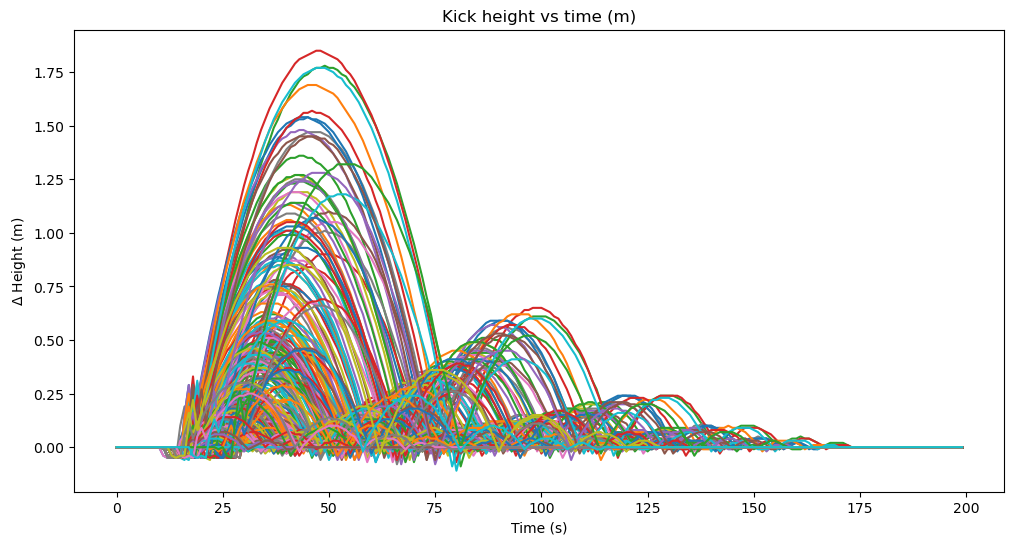
\includegraphics[width=14cm]{images/plotkicks.png}
\caption{Tracking dataset ground-truths}
\label{fig:plotkicks}
\end{center}
\end{figure}

The ground truth ball trajectories are plotted in \ref{fig:plotkicks} - which show a spectrum of different kicks have been captured. Two peculiar behaviors of the simulator's handling of the ball are noticed in the tracking data. Firstly, it is noted that at times the ball passes slightly through the ground of the pitch when it bounces. This is verified by comparing the rendered images to the logging and indeed seems to be the case although it is not understood why the simulation has this behavior. Secondly, the initial ball trajectory has a ``kink'' resulting from a slight non-physical change in position - which is caused by the server that does not execute a true kick, but rather instantaneously places the ball by the feet of the agent and then applies a velocity rather than performing a realistic kick, described by \cite{fatproxy}. This behavior only effects a minority of time-steps and is therefore accepted.

\begin{figure}[h!]
\begin{center}
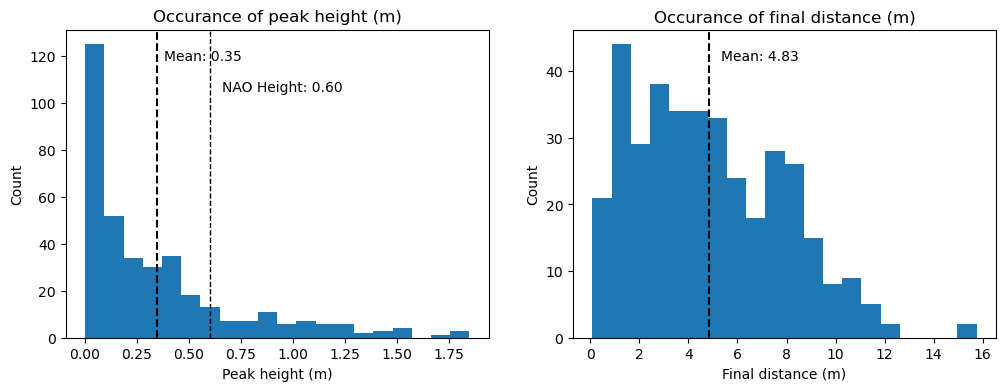
\includegraphics[width=16cm]{images/trackingplot.png}
\caption{Tracking dataset statistics}
\label{fig:trackplot}
\end{center}
\end{figure}

\section{Baseline tracking}

The baseline trackers, which have been chosen based on traditional methods popular in RoboCup as seen identified in the related works, are now investigated.

\subsection{Basic tracking}

Initially, the raw detections of the tracking dataset will be studied alongside the ground truth ball position as well as the ball position inferred by a perfect object detector. To do this, the ball detections are forward transformed to field ball positions using the same transformation as is used by the team, which has been extracted and captured in the meta data. A simple latch is then used for the most basic tracking, which means that missed and intermediate steps are filled by the previous positions.

\begin{figure}[h!]
\begin{center}
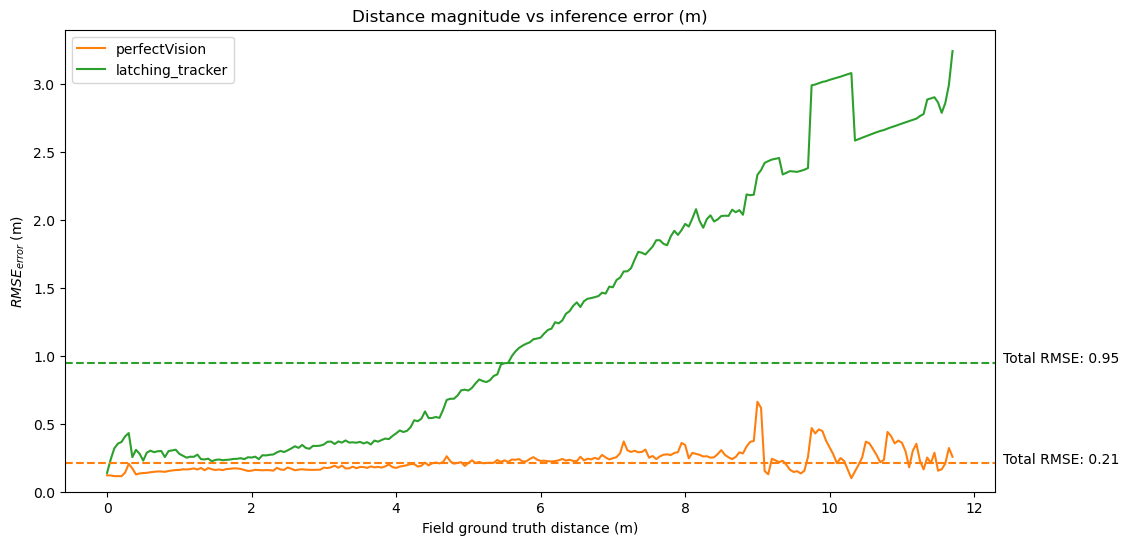
\includegraphics[width=14cm]{images/raw_error.png}
\caption{Basic tracking error}
\label{fig:rawerror}
\end{center}
\end{figure}

In figure \ref{fig:rawerror}, after forward transforming the bounding box to the field coordinates using the agents world model, the root mean square error is computed over binned kick distance. It can be seen from the error in the ``perfect vision'' that a ``noise floor'' exists due to the presence of inaccuracies in the forward transformation of the agent. A reason for this is that a simplified representation of the the agent model is presently used in the code base of the team which does not compensate for offsets in angular uprightness of the agent, which have generally been seen as providing an acceptable level of error compared to the complexity of a more accurate computation. Since the FatProxy agent walks on the spot when not commanded, the agent is constantly in motion and error is continuously introduced.

Near zero distance (before the Fat Proxy kick causes the ball beaming) the position error is dominated by the error in the transformation. This shows that the detector that has been trained is as effective as perfect vision up until the time of kicking. Up until approximately 4m distance from the agent, a portion of error can be assigned both the ball detector as well as the transformation model. Here the system works comparably to the performance suggested in the related works (tracking error of 0.3m) -- however the system has room for improvement although the improvement could equally be achieved by improving the transformation. However, beyond this point, it is evident that the error due to the detector explodes. Individual trajectories are investigated further in order to better understand this.

\begin{figure}[h!]
\begin{center}
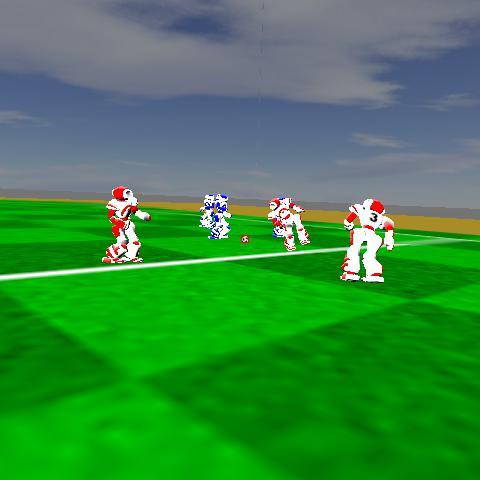
\includegraphics[width=8.5cm]{images/5mball.jpeg}
\caption{A ball at 5m distance}
\label{fig:farball}
\end{center}
\end{figure}

A short and long ground based kick is interrogated in figures \ref{fig:rawgroundshort} and \ref{fig:rawgroundlong}:

\begin{figure}[h!]
\begin{center}
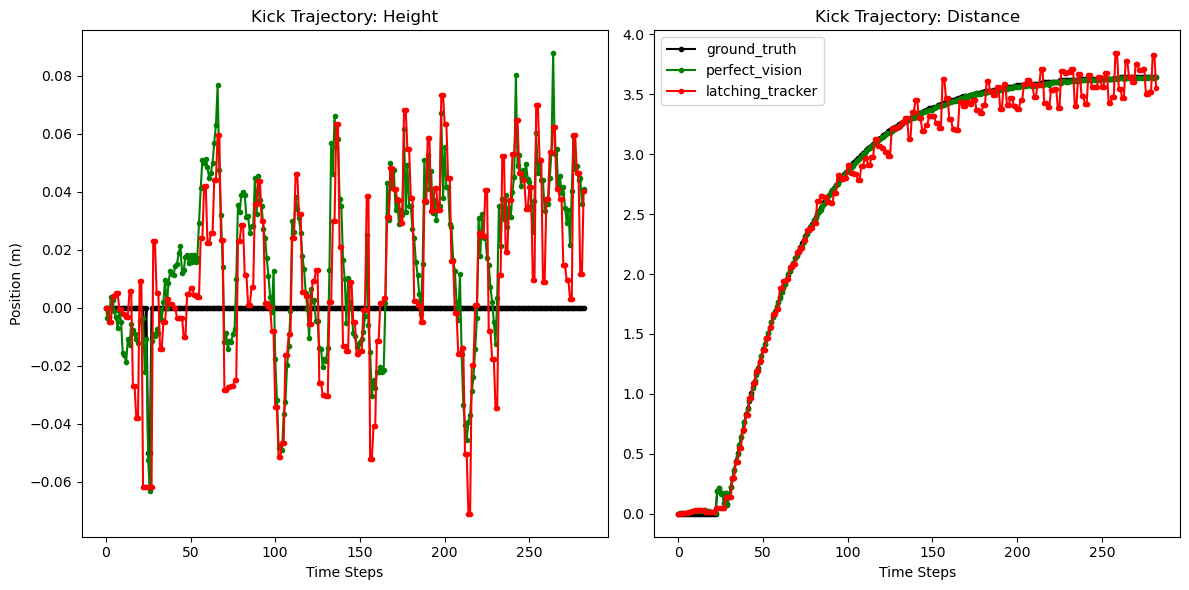
\includegraphics[width=14cm]{images/raw_ground_short.png}
\caption{Short ground kick - Raw detections}
\label{fig:rawgroundshort}
\end{center}
\end{figure}

\begin{figure}[h!]
\begin{center}
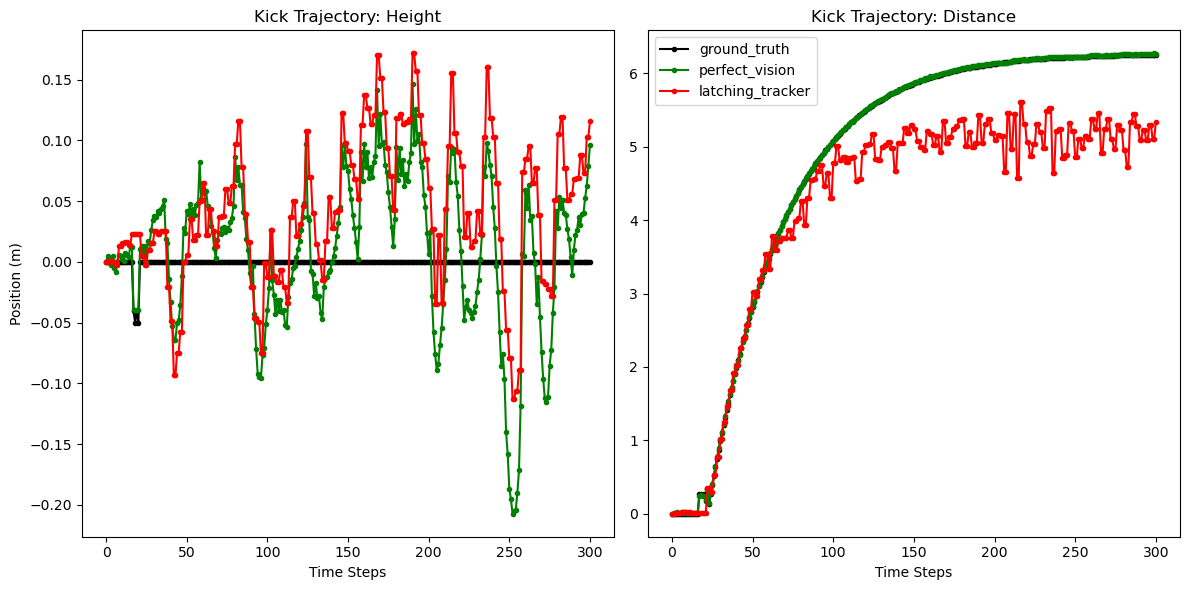
\includegraphics[width=14cm]{images/raw_ground_long.png}
\caption{Long ground kick - Raw detections}
\label{fig:rawgroundlong}
\end{center}
\end{figure}

In these kicks the following is noted. Firstly, looking at the ground truth trajectory for a kick along the ground the height of the ball remains zero as expected. The distance covered by the ball per unit time decreases in a non-linear manner after the kick takes place, due to rolling friction. Secondly, looking at the measurements of the trajectory there is noise introduced by the detector and transformation which here can be observed in the time domain, where it is clear that the cyclic nature of the agent motion results in an error in the perceived ball height. The correctness of the height has a dependency on the placement of the bounding box, which appears to be comparable to the perfect object detector. Until 4m the inference of distance appears to be effective, although noisy. Beyond this distance, inference of the ball position appears to be problematic. Since accuracy of the distance is dependent on the size of the bounding box, it seems that a limit exists. The object detector is impressive within it's reliable range.

A short and long lofted kick is interrogated in figures \ref{fig:rawloftshort} and \ref{fig:rawloftlong}:

\begin{figure}[h!]
\begin{center}
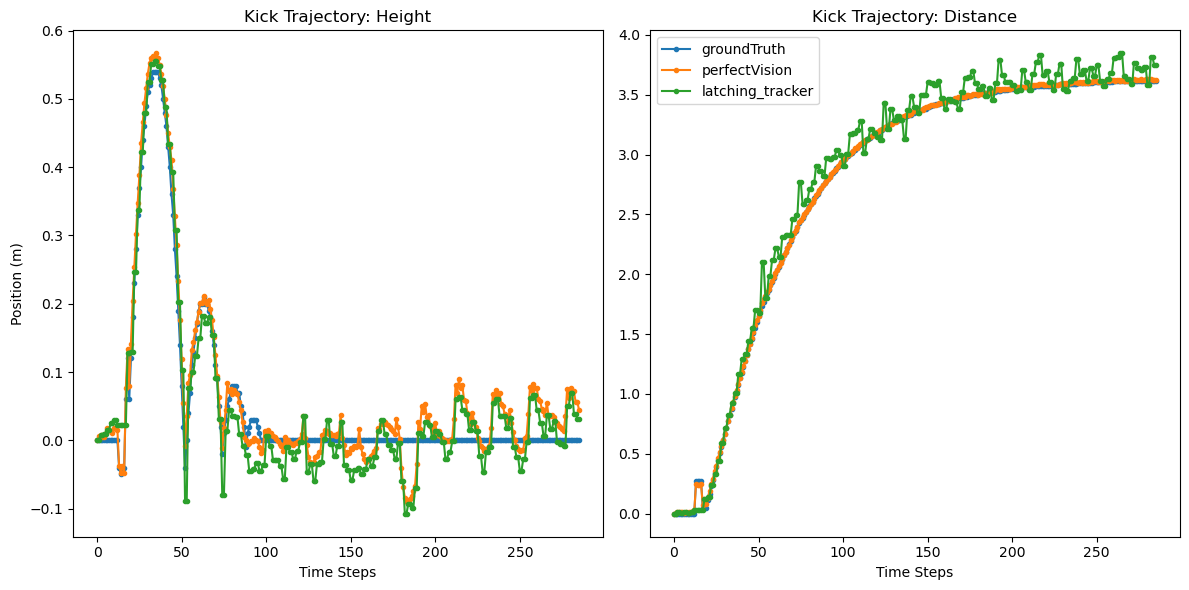
\includegraphics[width=14cm]{images/raw_loft_short.png}
\caption{Short lofted kick - Raw detections}
\label{fig:rawloftshort}
\end{center}
\end{figure}

\begin{figure}[h!]
\begin{center}
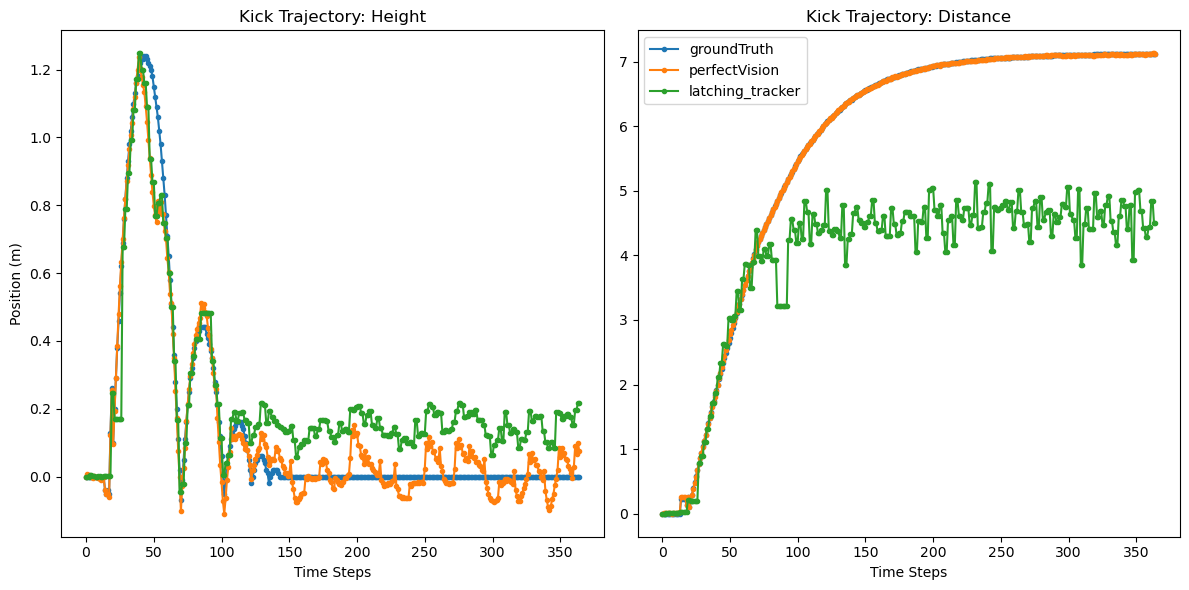
\includegraphics[width=14cm]{images/raw_loft_long.png}
\caption{Long lofted kick - Raw detections}
\label{fig:rawloftlong}
\end{center}
\end{figure}

For lofted kicks, it is firstly noted that the trajectory follows a parabolic path as expected for projectile motion. With each bounce, energy losses causes rebounds of diminishing height. Secondly it is noted that within 4m the detector is comparable to perfect vision. Beyond 4m a limit on the ball distance is reached which causes the error to explode. 

The distance measurement at long range is the limiting factor for the overall performance of the system - in figure \ref{fig:farball} it is understandably so since the ball becomes tiny, therefore any changes in distance are difficult to perceive. However, early detections are reliable, therefore applying a tracking algorithm has the potential to improve the tracking of the ball trajectory. 

\subsection{Standard Kalman Filtering}

Initially, a simplistic approach is taken by assuming the process (the ground motions of the ball) can be described by Newton's famous equations of motion - as a constant velocity model in equation \ref{eqn:newton} below. This dynamics model can then be expressed as a linear set of recursive equations as follows in equation \ref{eqn:firstorder}:

\begin{equation} 
x_k=v\Delta t + x_{k-1}
\label{eqn:newton}
\end{equation}
\begin{equation} 
x_k
=
F(t)x_{k-1}
=
\begin{bmatrix}
    1 & \Delta t \\
    0 & 1 
\end{bmatrix}
x_{k-1}
\label{eqn:firstorder}
\end{equation}

Applying the constant velocity model in the prediction step of a Kalman filter results in what is known as a ``first order'' Kalman filter, where a zero order filter assumes constant position. The measurement noise $R$ must be assumed to be of Gaussian nature and is quantified by comparing it to the error of all the measurements taken to the respective ground truths. The process noise model $Q$ assumes zero-mean white noise of a Gaussian nature, originating as fluctuations in the velocity. A continuous velocity noise model $Q_c$ (equation \ref{eqn:cnoise}) can be discretized for the desired time step and propagated through the system dynamics model $F$ using equation \ref{eqn:dnoise}. \citep{kalmanpy}

\begin{equation} 
Q_c
=
\begin{bmatrix}
    0 & 0 \\
    0 & 1 
\end{bmatrix}
\Phi
\label{eqn:cnoise}
\end{equation}
\begin{equation} 
Q = \int\limits_0^{\Delta t} F(t)Q_cF^T(t)dt
=
\begin{bmatrix}
    \Delta t^3/3 & \Delta t^2/2 \\
    \Delta t^2/2 & \Delta t 
\end{bmatrix}
\Phi
\label{eqn:dnoise}
\end{equation}

$\Phi$ is the spectral density of the white noise - which is often difficult to compute or measure, especially when the process model differs from reality and is therefore often applied as an engineering factor or found by tuning. In order to find an appropriate $\Phi$ for the ball tracking task, a search is used. The results are shown in figures \ref{fig:fokgroundshort} and \ref{fig:fokgroundlong}.

\begin{figure}[h!]
\begin{center}
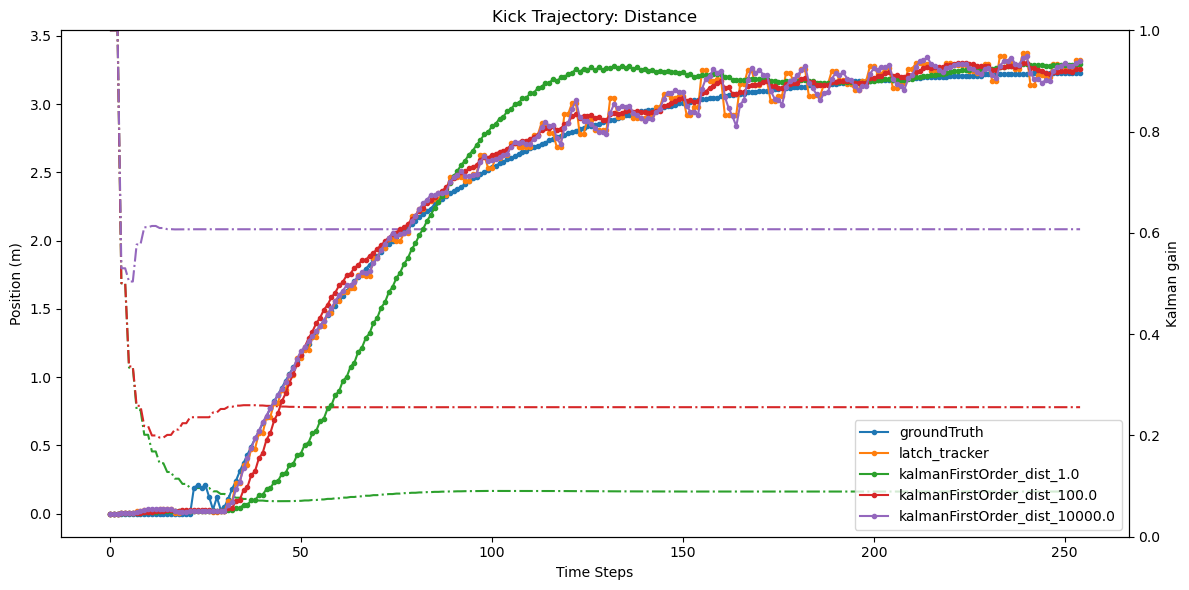
\includegraphics[width=12cm]{images/fok_ground_short.png}
\caption{Short ground kick - First order Kalman Filter search}
\label{fig:fokgroundshort}
\end{center}
\end{figure}

\begin{figure}[h!]
\begin{center}
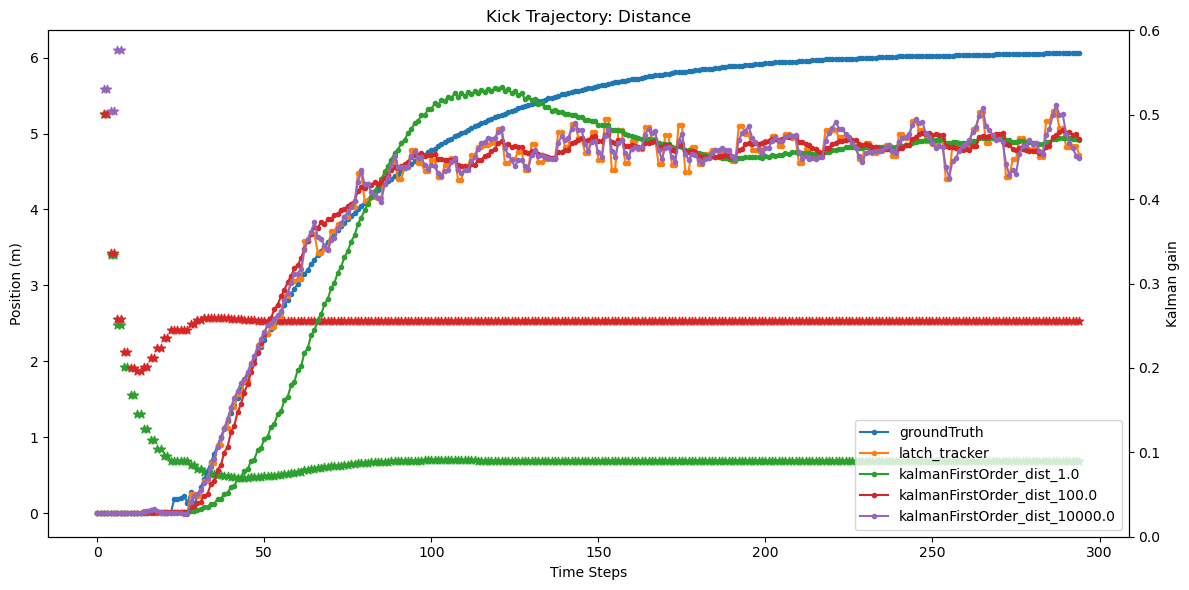
\includegraphics[width=12cm]{images/fok_ground_long.png}
\caption{Long ground kick - First order Kalman Filter search}
\label{fig:fokgroundlong}
\end{center}
\end{figure}

%\begin{figure}[h!]
%\begin{center}
%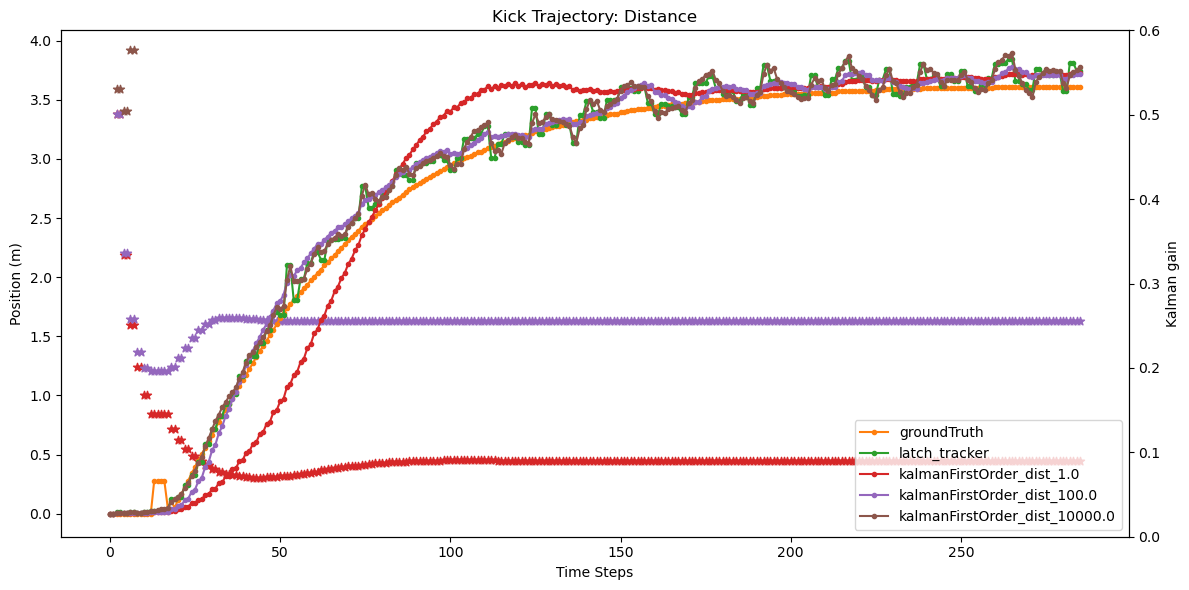
\includegraphics[width=12cm]{images/fok_loft_short.png}
%\caption{Short lofted kick - First order Kalman Filter search}
%\label{fig:fokloftshort}
%\end{center}
%\end{figure}

%\begin{figure}[h!]
%\begin{center}
%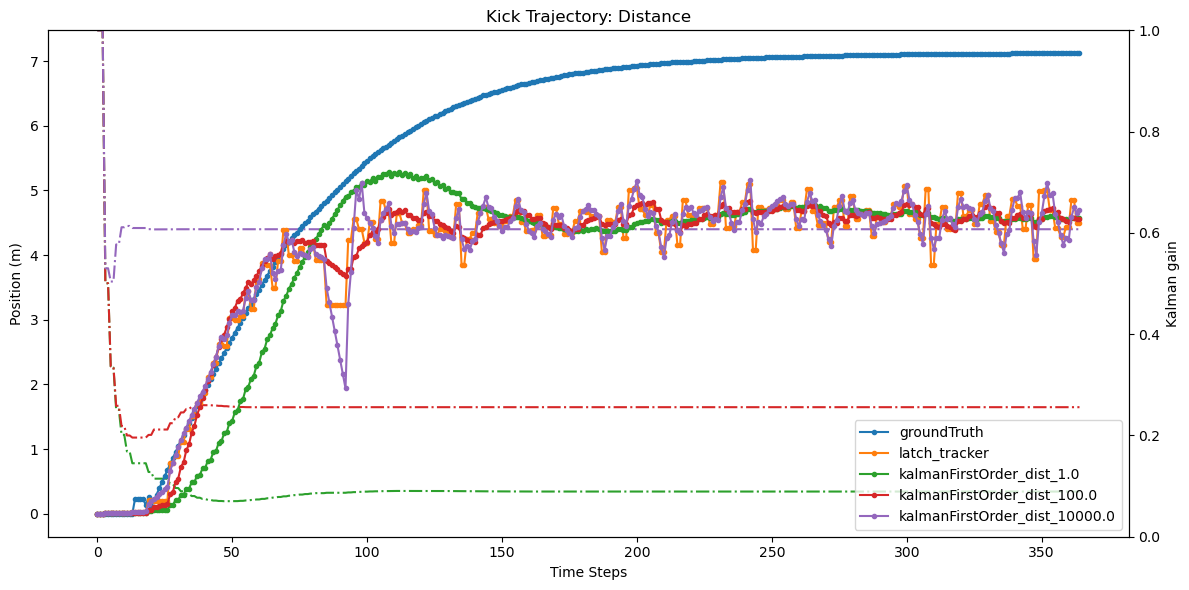
\includegraphics[width=12cm]{images/fok_loft_long.png}
%\caption{Long lofted kick - First order Kalman Filter search}
%\label{fig:fokloftlong}
%\end{center}
%\end{figure}

By inspecting a set of kicks, one can get an understanding of the characteristics of the first order Kalman tracker. Initially, at the start of each kick, the model uncertainty is initialized high which results in a Kalman gain close to 1. This corresponds to a strong dependency on the sensor measurement (rather than the prediction model) which helps to obtain a better initial state estimation. This makes sense as initially there is an assumption of no knowledge of the object states. As time steps are performed the Kalman gain reduces and the model relies less on the measurement and more on the dynamics model, which can result in noise attenuation. The rate of convergence is an intrinsic property of the model -- it is not ``intelligent'' and relies on timing -- and in this case convergence happens before the ball is kicked which means that the constant velocity assumption causes a significant lag when it is strongly relied upon.

The ultimate steady state of the Kalman gain depends on the balance of the magnitudes of the measurement noise and process uncertainty. When the process is very uncertain (high $\Phi$) then the filter tends to ignore the dynamics model and a state estimation with negligible difference from a no filtering approach is achieved. As $\Phi$ is reduced, the dynamics model plays a larger role. With prior knowledge that the object is moving at constant velocity, it is possible to attenuate noise. However, if the dynamics model is overly dominant it causes a lag in the cases where the ball does not behave as is modeled by the function. This can lead to significant error, much worse than if no filtering is applied. There exists a trade off between responsiveness and noise attenuation.

\begin{figure}[h!]
\begin{center}
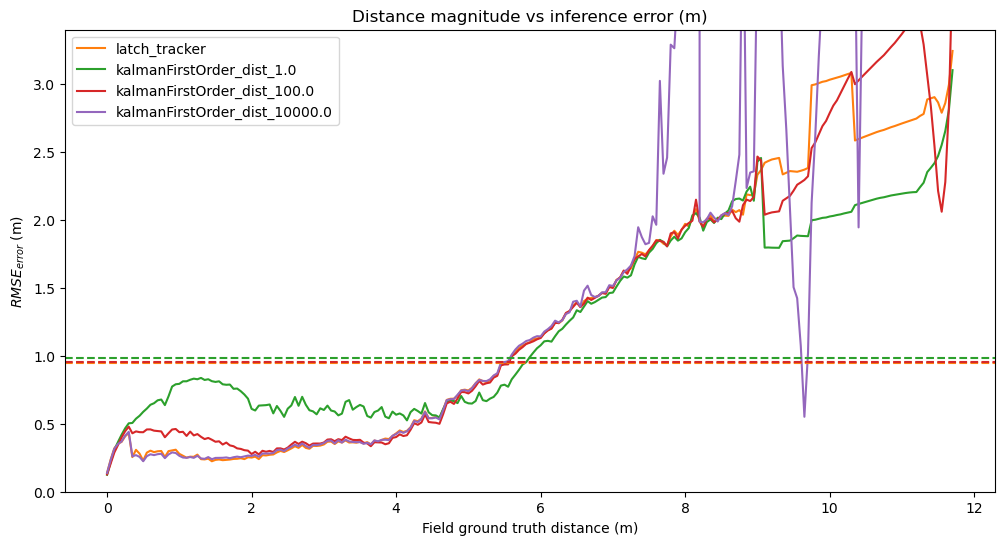
\includegraphics[width=14cm]{images/fok_error.png}
\caption{First order Kalman Filter error}
\label{fig:fokerror}
\end{center}
\end{figure}

The tracking error has been plotted in figure \ref{fig:fokerror}. Although the filter can be tuned in order to achieve some noise attenuation, the Kalman filter assumes Gaussian noise with a zero mean and is therefore is not able to capture the heavily non-linear characteristics of the distance measurement. Therefore, the standard Kalman filter is not able to learn and compensate for the large non-linearity which in this cases dominates the error significantly more than the position jitter. It can be seen in figure \ref{fig:fokerror} that for such a complex case, the application of a standard first order Kalman filter, across a variety of $\Phi$, is either detrimental or causes negligible improvement to the performance compared to no tracking being used.

\subsection{Extended Kalman Filtering}

A more sophisticated model describing the ground motion of the ball, which has been successful in the RoboCup domain, is described by \cite{kalmanmodel} where it was first applied to their team (CMUnited) to win the RoboCup-97 small-robot competition. As per \cite{kalmanmodel}, the rolling resistance of a ball can be expressed by a constant (but unknown) discounting factor $\lambda$ which is defined as a state variable and iteratively applied in order reducing velocity each time step by a constant descaling. This dynamics model can then be expressed as a non-linear set of recursive equations as follows in equation \ref{eqn:dragorder} - which can be applied in an Extended Kalman filter:

\begin{equation} 
\begin{bmatrix}
    x_{k+1} \\
    \dot{x}_{k+1} \\
	\lambda_{k+1} \\
\end{bmatrix}
=
\begin{bmatrix}
    x_{k} + \dot{x}_{k} \cdot \Delta t\\
    \dot{x}_{k} \cdot \lambda_{k} \\
	\lambda_{k} \\
\end{bmatrix}
\label{eqn:dragorder}
\end{equation}

The same measurement noise $R$ is applied, as for the first order Kalman filter, as is the same process noise model $Q$. Again $\Phi$ is to be found by doing a search (figures \ref{fig:ekfgroundshort} and \ref{fig:ekfgroundlong}.

\begin{figure}[h!]
\begin{center}
\includegraphics[width=11cm]{images/ekf_ground_short.png}
\caption{Short ground kick - Extended Kalman Filter}
\label{fig:ekfgroundshort}
\end{center}
\end{figure}

\begin{figure}[h!]
\begin{center}
\includegraphics[width=11cm]{images/ekf_ground_long.png}
\caption{Long ground kick - Extended Kalman Filter}
\label{fig:ekfgroundlong}
\end{center}
\end{figure}

%\begin{figure}[h!]
%\begin{center}
%\includegraphics[width=12cm]{images/ekf_loft_short.png}
%\caption{Short lofted kick - Extended Kalman Filter}
%\label{fig:ekfloftshort}
%\end{center}
%\end{figure}

%\begin{figure}[h!]
%\begin{center}
%\includegraphics[width=12cm]{images/ekf_loft_long.png}
%\caption{Long lofted kick - Extended Kalman Filter}
%\label{fig:ekfloftlong}
%\end{center}
%\end{figure}

The EKF operates in a similar fashion to the standard Kalman filter. Initially the Kalman gain is set close to 1 and it converges (unintelligently) towards a steady state which is dependent of the balance between measurement and process noise. In the case of an EKF however there is some instability, due to the nonlinearity of the process model, which causes the Kalman gain to oscillate in some cases. Compared to the first order Kalman filter, it is seen that after the initial kick that the tracker has a reduction in overshoot. The model is therefore more responsive and can in principle be more aggressively tuned for noise rejection.

\begin{figure}[h!]
\begin{center}
\includegraphics[width=12cm]{images/ekf_error.png}
\caption{Extended Kalman Filter error}
\label{fig:ekferror}
\end{center}
\end{figure}

Although a more sophisticated approach, in figure \ref{fig:ekferror} the EKF still suffers from some of the same simplistic assumptions as used for the first order Kalman filter. The EKF is not an optimal tracker for this case and therefore is either detrimental or causes negligible improvement to the performance compared to no tracking being used.

\newpage
\section{Proposed tracking}

For the tracking cases considered it is apparent that the performance is sub optimal. Neural Kalman filtering is an approach to Kalman filtering which can be used when the underlying state space model is non-linear and acccurate knowledge of it is unknown. In this section the application of neural Kalman filtering to the tracking problem is investigated.

\subsection{Changes to KalmanNet}

Initially the KalmanNet Github repository \cite{kalmangit} is cloned and it is attempted to reproduce their training results and then begin training for the ball tracking problem. Various issues were encountered which made training impractical therefore some changes were applied. The targeted major issues were: frequent cases of overflow in training following initialization (models which diverge immediately), impractically slow convergence (across learning rates) as well as high ultimate loss scores. Therefore the useful basic structure of the KalmanNet repository and training routine is utilized but some changes which significantly improved performance for this research has been implemented to achieve practical neural Kalman filtering. 

Although some of the KalmanNet architecture is peculiar, some of the choices are not necessarily improper but they simply seemed to just do not work well for the research problem being considered here. They may still have useful results in other domains:
\begin{itemize}
    \item In figure \ref{fig:architecture} it is shown that the predicted Kalman gain results from a fully connected linear output layer. Although its not necessarily an invalid approach, it does however not conform to the essence of Kalman filtering where the Kalman gain must lie between 0 and 1 - which has an intuition of describing a level of confidence in the measurements. Therefore it is chosen to replace this layer with a softmax layer, which has the effect of clamping the range. It was found that this change immediately solved the instability of the model and significantly increased the rate of convergence.
    \item In both the \cite{kalmannet} paper as well as in figure \ref{fig:blockd}, the data preprocessing step is not fully described. It is found that the input features are scaled by the magnitude of the state vector. This introduces significant non-linearity to the problem since with this processing, for example, at zero velocity the model would have the same input feature (state estimate and measurement) at a position of 0m as it would as a position of 1000m. This has the effect of destroying necessary information for this research problem being considered. A minimalistic approach was applied by simply applying an identity transformation to the input features and relying on the linear input layer with applied bias -- which was found to give sufficient results for this dataset without relying on prior knowledge -- and notably boosted the ultimate performance of the model by achieving a lower loss than using the existing feature. Empirically this gave better training results compared to other approaches taken such as standardization and normalization.
\end{itemize}


\subsection{Model training}

In order to use the KalmanNet model training routine, a data loader must be constructed which creates the expected data structure in a tensor format. The duration of each kick must be uniform in order to fit in the data structure, therefore it is decided to clip all kicks at 230 time steps, which corresponds to the shortest kick in the training dataset. The GRU is reset only per epoch, which aims to prevent over fitting on the moment of starting the kick as well as reducing the importance of timing initialization. To train the network, the mean square error is minimized with cross validation applied to store the best model weights found.

Compared to the CNN models trained previously, significantly slower processing of the data was realized -- which is most likely due to the sequential nature of the problem and data. A speed up was achieved (more than an order of magnitude over CPU) by training utilizing NVIDIA GeForce RTX 3090 processors, which still resulted in a training time of nearly 12 hours per model for 1000 Epochs. Apart from being impractical, is not believed that longer training of this model would deliver better results. Training results were found be highly variable and the results of each trained model differed significantly. By training numerous models with the same parameters, it was possible to select the best one. The results of two trained models (best and cherry picked) are plotted in figure \ref{fig:RNNtrain} in order to convey the variety in training seen.

\begin{figure}[h!]
\begin{center}
\includegraphics[width=9.5cm]{images/knet_train.png}
\caption{Neural network adided Kalman filtering model training}
\label{fig:RNNtrain}
\end{center}
\end{figure}

At initialization the model scores extremely poorly, however, rapidly converges on a lower loss score for against both the training and cross validation score. This is a good indication that the model is learning and capturing patterns within the data. The fact that both training and validation scores are indiscernibly close provides confidence that the model is not over-fitting on the training data. Between the two models shown, further epochs lead to either further convergence or even divergence depending on the learning of the model. The best model achieves its performance after 612 epochs with further training resulting in diminishing performance.

\subsection{Evaluation of results}

The trackers that have been considered thus far are now evaluated against the unseen test training set. In order to have a feel for the results - a representative short and long grounded kick are interrogated in figures \ref{fig:evalgroundshort} and \ref{fig:evalgroundlong}. In particular the focus is on understanding the performance of the neural aided tracking method as well as how it compares to the traditional approaches.

\begin{figure}[h!]
\begin{center}
\includegraphics[width=12cm]{images/eval_ground_short.png}
\caption{Short ground kick - Tracker evaluation}
\label{fig:evalgroundshort}
\end{center}
\end{figure}

\begin{figure}[h!]
\begin{center}
\includegraphics[width=12cm]{images/eval_ground_long.png}
\caption{Long ground kick - Tracker evaluation}
\label{fig:evalgroundlong}
\end{center}
\end{figure}

%\begin{figure}[h!]
%\begin{center}
%\includegraphics[width=12cm]{images/eval_loft_short.png}
%\caption{Short lofted kick - Tracker evaluation}
%\label{fig:evalloftshort}
%\end{center}
%\end{figure}

%\begin{figure}[h!]
%\begin{center}
%\includegraphics[width=12cm]{images/eval_loft_long.png}
%\caption{Long lofted kick - Tracker evaluation}
%\label{fig:evalloftlong}
%\end{center}
%\end{figure}

Initially, at the start of the kick routine, the neural network predicts Kalman gains close to 1 -- which is a desirable initialization behavior. This is also shared and considered to be a highly effective feature of the standard Kalman and EKF trackers. This also corresponds to the knowledge that the early measurements are reliable and shows that meaningful learning has occurred. Compared to the standard and EKF trackers however, the neural assisted method does not show an initial convergence of the gain. Due to this, it can be recognized, that when the kick is performed the neural Kalman filter does not show any lag in the same manner as the traditional methods do, which have already converged. Since the traditional trackers have a portion of a mismatching physics model as part of the update, these models will always experience a lag.

At close range, after agent has performed the kick, the Kalman gain remains consistent but is not static. In this manner the state estimation benefits from accurate measurements and retains responsiveness. As the ball travels further in distance within the region of reliable detection the rolling average Kalman gain drops only slightly. With a gain near 1, the neural Kalman filter tracks the trajectory similarly, but slightly ahead of, the latch tracker (a reflection of the raw detections) rather than the ground truth. An explanation for a lack of learning here is likely that the loss resulting from such a case is very small compared to the loss from range limited detections. This may also explain why there seems to be no noise attenuation -- the error reduction is imperceptible.

In figure \ref{fig:evalgroundlong} the impacts of the ball moving into the longer range region is seen. It is apparent that as the ball moves into the region where the detection become range limited that the Kalman gain predictions start to become interesting. A sudden onset of high frequency jumps in the Kalman gain appear, which has the effect of increasing the state estimate beyond the measured distance. The result of this is that the state estimate diverges from the measurements. The mechanism for this appears to be that certain measurements are ``extrapolated'' upwards by the first order Kalman filter by dropping the gain. A high Kalman gain then corrects for an overshoot by using the measurement to drop the state estimation. In this manner, the amplitude of the fluctuations might be understood as a measure of uncertainty. A side effect of this is that it results in an amplification of the jitter resulting from the measurement noise.

As more time steps are elapsed and velocity of the ball starts to reduce the rolling average Kalman gain drops further -- this places a greater emphasis on the dynamics model. The effect of this is that despite more range limited measurements arriving, the state estimations are able to track the ground truth rather than converging on the measurements as with the traditional tracking methods. A complex behavior appears been learnt where the tracker has been able to capture the trajectory of the ball despite the range limited measurements. In this manner it does appear that the network has indeed implicitly learnt to capture the underlying system dynamics. 

The error of the trackers against the unseen test data is plotted in figure \ref{fig:evalerror}:

\begin{figure}[h!]
\begin{center}
\includegraphics[width=13cm]{images/eval_error.png}
\caption{Tracker error (Test set)}
\label{fig:evalerror}
\end{center}
\end{figure}

Overall it can be seen that of all the trackers considered, neural Kalman filtering has achieved the lowest root mean square error against the test dataset. The majority of the performance gain arises from an improved tracking from the long kicks which travel beyond the range where the object detector is reliable. In this region the neural network has implicitly captured the underlying system dynamics which facilitates divergence of the state estimation from the measurements accordingly. Neural Kalman filtering is also the most responsive tracking approach, having a reduced error in the region up to 1m after the kick due to a reduction in latency when the process diverges from the dynamics model. 

With the model that has been utilized there are however aspects which come at a cost of the previously mentioned performance. In the region where the detections are accurate, the traditional approaches track better. A possible explanation is that the loss scores due to this error are small in comparison to the error from the range limited measurements. Therefore, during training, the network does not learn to optimize Kalman gain predictions in the middle range regions. Another cost is noise amplification, which seems to manifest due to the fluctuations in the Kalman gain predictions as the network has some level of uncertainty.

In order to evaluate the real-time performance of the tracking algorithms, a bench-marking of the trackers is performed and plotted in figure \ref{fig:trackspeeds}:

\begin{figure}[h!]
\begin{center}
\includegraphics[width=7.5cm]{images/tracker_speeds.png}
\caption{Tracker speeds}
\label{fig:trackspeeds}
\end{center}
\end{figure}

All algorithms are have been implemented in Python and tested on a mobile laptop CPU as done with the evaluation of object detectors. In \ref{fig:trackspeeds} it is seen that the simple latch tracker is the best performing approach in terms of computational speed. At such frequencies, the measurement error is likely significant however is useful for relative comparison. The standard Kalman filter and EKF tracker have a diminished speed respectively due to increased complexity. Neural network aided Kalman filtering is two orders of magnitude slower than the latch, however, still completes multiple orders of magnitude faster than the object detectors. Therefore the tracking step is not limiting and completes in real time despite the addition of further complexity. 

%%%%%%%%%%%%%%%%%%%%%%%%%%%%%%%%%%%%%%%%%%%%%%%%%%%%%%%%%%%%%%%%%%%%%%%%%%%%%%%%%%%%%%%%%%%%%%%%
\chapter{Conclusion}

The aim of visual object tracking is to use a sequence of image frames to robustly estimate the motion state of a target object. This offers a versatile approach that is capable of acquiring an abundance of environmental information that can be used by robotic agents to perceive and interact with a dynamic environment in real-time. In this research report, the context of ball tracking in a simulated RoboCup soccer environment is considered. It has been proposed to take advantage of the progress of modern neural approaches to computer vision by utilizing models from the popular problem space of object detection by utilizing a tracking-by-detection framework. Correspondence can then be achieved through the the use of Kalman filtering which is a popular model based commonly used for state-estimation in the robotics domain. It was proposed to apply neural assisted Kalman filtering, which balances the ease of interpretation of a model-based approach and the ability to learn complex dynamics using neural networks. 

For the object detection task, the findings of the research showed that


\subsubsection{Reflection}

After training and evaluating the various detectors, the principle questions of the object detection study can be addressed. Firstly, it is clear that pretraining on real images can indeed be transferred to a simulated RoboCup environment - with the pretrained object detectors that are trained on COCO managing to achieve useful scores and even outperforming trained VJ detection. Further, it is clear that CNN object detectors can run at real-time on a modern mobile CPU and achieve useful performances. Both the YOLO v4 Tiny as well as NanoDet can be trained for real-time speeds and achieve useful inference which can be used on a robotics platform. Most significantly, the more recent key point based NanoDet detector outperforms the popular YOLO v4 Tiny and and traditional VJ detectors as measured by AP at real-time speed. Finally, it is seen that model quantization can indeed cause a noticeable performance degradation, with the reduction in model size not yielding a worthwhile return to justify its inclusion. 

For the tracking task, the findings of the research showed that. The results are in line with the observations of \cite{diagnosingtrack}, who suggests that the performance of visual object trackers are dominated by their ability to perform feature extraction.

Moldel mismatch. Learn complex dynamics

Addition of PAN

\section{Future work}

In this subsection some potential areas for further investigation are discussed which follow the observations and results of the research. 

\subsection{Improving ball measurements}

Although the performance of the object detectors on detecting a distant ball was more impressive than expected, there is room for improvement of the bounding box regression which appears to have a minimum size limit despite still being able to make successful ball classifications. A reason for this may be found in the architecture of the Path Aggregation Network, which leverages the pyramidal hierarchy of the network backbone in order to combine higher and lower level feature maps which represent semantic and spacial information accordingly as seen in figure \ref{fig:pan}. 

\begin{figure}[h!]
\begin{center}
\includegraphics[width=10cm]{images/pan.jpg}
\caption{Path Aggregation Network \citep{pan}}
\label{fig:pan}
\end{center}
\end{figure}

The largest feature map that is laterally connected has undergone down-scaling due to the stride of the CNN backbone. Therefore, in order to improve the bounding box regression, a higher resolution feature map may boost regression by supplementing additional spatial information. In NanoDet a stride of 8 is used, however, reducing the stride is undesirable for real-time performance since -- due to the arithmetic complexity of the CNN -- in order to achieve a bottle neck of the same ultimate feature map size with a reduced stride by factor $a$, an expansion of the number of computations proportional to $a^3$ would result which would impact the detector real-time performance. In the simplest approach one might resize the image by a factor $8$, however this creates $8^2$ more computations in the backbone. A potential approach that adds only a small overhead would be the addition of an additional up-sampling layer, with a lateral connection to the input layer.

Constrained to monocular vision, in order to further improve the distance measurement -- after having computed a bounding box -- it may be possible to use further clues such as optical methods or environmental information. One optical approach may be to utilize the phenomenon of motion parallax  where an observation from two different points leads to an apparent displacement of an object. In this manner the natural sideways bobbing of the agent can give depth information -- similar in the same manner as one sees in nature from pigeons \citep{parrelax}. Further environmental observations such as the position of the ball against field markings as well as the perceived gravitational drop of a ball, if it is a lofted kick, can give additional information in the correct circumstances.

\subsection{Improving state estimation}

Although neural Kalman filtering was able to outperform the traditional tracking methods as measured by MSE -- there are some issues which should be addressed. 

One issue is that, within the reliable range of the object detector, the neural based approach underperforms versus the traditional methods. It is more desirable to have a tracker which is best across the range rather than specializing for certain circumstances. The current issue appears to be that the region where the detector is reliable does not contribute significantly to the loss score. Therefore, applying a focal loss inversely based on distance may encourage a better performance in this region (possibly at a cost at the long range which might be tuned using a hyper-parameter). Alternatively, a loss based on integrated error (similar in nature to the integral gain of a PID controller) may help to reduce the steady state error which will also boost the performance in this region.  

A further issue is the impact of jitter, which is undesirable for control purposes. Traditional Kalman filters are often used to provide some noise attenuation in a signal. The neural Kalman filter used in this research however has a tendency to add additional noise. One approach may be to punish volatility using a loss metric of sorts, however, this may have ill consequences since punishing rapid change is likely to result in the loss of responsiveness. The fluctuations also seemed to be related to an expression of uncertainty, punishing this may result in a degradation of performance. Therefore a better way may to to rather add a component dedicated to smoothing within the end-to-end model. This might be a traditional Kalman filter (or more sophisticated filter).

\subsection{Extensions}

Additional further work is considered below:

An aspect which has not been considered in this research is the ability of the model to predict the future time steps. This can be useful for agent positioning. Forward predictions from a Kalman filter are usually performed by skipping the correction step. In the case where the dynamics model is significantly different from the process, the prediction will diverge significantly from the real process which can be significantly more complex in the case of neural Kalman filtering. In order to get useful future predictions for ball tracking, replacing the embedded first order Kalman filter with an EKF model is an approach which will yield better predictions but should also improve the tracking accuracy as the model better represents the underlying dynamics. However, due to the additional complexity, may add further complexity to training. An alternative approach would be to create a recurrent model to predict the future measurements.

A limitation of the approach used in this research is that a pipeline between detection and tracking is utilized rather than end-to-end training. Due to this, the detection loss is not the same as the ultimate metric which is used to evaluate the tracker. A benefit of this approach is that there is modularity in the system -- a newly trained object detector model could be substituted in without requiring retraining of the tracker. Further, other visual systems (such as for agent localization) can plug in to use the results without further complicating training. A consequence of this is that the detector not actually optimized specifically for the tracking task, so there is potentially additional performance which can be gained here. An approach might be taken which would train end-to-end, utilizing a common backbone with different heads for each of the desired tasks, would could result in better performances but at a cost of complexity and further loss of intuition.

The natural continuation of this work would be to apply the detection and tracking to a physical robotic system in a real world setting. For detections it is interesting to investigate how well the detectors generalizes to the real world with various natural sources of optical noise as well as scene variation in both the foreground (different balls) and the background. For, tracking there will be significantly more variation possible especially on a natural pitch where wind, spin and an imperfect surface can result in changes to the ball trajectory. Transfer learning might be investigated in order to reduce the effort required to create a sufficiently descriptive dataset.s

%%%%%%%%%%%%%%%%%%%%%%%%%%%%%%%%%%%%%%%%%%%%%%%%%%%%%%%%%%%%%%%%%%%%%%%%%%%%%%%%%%%%%%%%%%%%%%%%
%\appendix
%\chapter{Appendix}\label{app:extra}
%Appendix A
%
%\section{Section 1}\label{app:whatis}
%Section 1

%%%%%%%%%%%%%%%%%%%%%%%%%%%%%%%%%%%%%%%%%%%%%%%%%%%%%%%%%%%%%%%%%%%%%%%%%%%%%%%%%%%%%%%%%%%%%%%%
%\chapter{Appendix}\label{app:extra}
%Appendix B

%\section{Section 1}\label{app:whatis}
%Section 1

%%%%%%%%%%%%%%%%%%%%%%%%%%%%%%%%%%%%%%%%%%%%%%%%%%%%%%%%%%%%%%%%%%%%%%%%%%%%%%%%%%%%%%%%%%%%%%%%
\bibliography{references}\addcontentsline{toc}{chapter}{References}
\end{document}
